\documentclass[12pt,brazil]{article}\usepackage[]{graphicx}\usepackage[]{xcolor}
% maxwidth is the original width if it is less than linewidth
% otherwise use linewidth (to make sure the graphics do not exceed the margin)
\makeatletter
\def\maxwidth{ %
  \ifdim\Gin@nat@width>\linewidth
    \linewidth
  \else
    \Gin@nat@width
  \fi
}
\makeatother

\definecolor{fgcolor}{rgb}{0.345, 0.345, 0.345}
\newcommand{\hlnum}[1]{\textcolor[rgb]{0.686,0.059,0.569}{#1}}%
\newcommand{\hlsng}[1]{\textcolor[rgb]{0.192,0.494,0.8}{#1}}%
\newcommand{\hlcom}[1]{\textcolor[rgb]{0.678,0.584,0.686}{\textit{#1}}}%
\newcommand{\hlopt}[1]{\textcolor[rgb]{0,0,0}{#1}}%
\newcommand{\hldef}[1]{\textcolor[rgb]{0.345,0.345,0.345}{#1}}%
\newcommand{\hlkwa}[1]{\textcolor[rgb]{0.161,0.373,0.58}{\textbf{#1}}}%
\newcommand{\hlkwb}[1]{\textcolor[rgb]{0.69,0.353,0.396}{#1}}%
\newcommand{\hlkwc}[1]{\textcolor[rgb]{0.333,0.667,0.333}{#1}}%
\newcommand{\hlkwd}[1]{\textcolor[rgb]{0.737,0.353,0.396}{\textbf{#1}}}%
\let\hlipl\hlkwb

\usepackage{framed}
\makeatletter
\newenvironment{kframe}{%
 \def\at@end@of@kframe{}%
 \ifinner\ifhmode%
  \def\at@end@of@kframe{\end{minipage}}%
  \begin{minipage}{\columnwidth}%
 \fi\fi%
 \def\FrameCommand##1{\hskip\@totalleftmargin \hskip-\fboxsep
 \colorbox{shadecolor}{##1}\hskip-\fboxsep
     % There is no \\@totalrightmargin, so:
     \hskip-\linewidth \hskip-\@totalleftmargin \hskip\columnwidth}%
 \MakeFramed {\advance\hsize-\width
   \@totalleftmargin\z@ \linewidth\hsize
   \@setminipage}}%
 {\par\unskip\endMakeFramed%
 \at@end@of@kframe}
\makeatother

\definecolor{shadecolor}{rgb}{.97, .97, .97}
\definecolor{messagecolor}{rgb}{0, 0, 0}
\definecolor{warningcolor}{rgb}{1, 0, 1}
\definecolor{errorcolor}{rgb}{1, 0, 0}
\newenvironment{knitrout}{}{} % an empty environment to be redefined in TeX

\usepackage{amsmath}
\usepackage{alltt}
\usepackage{babel}
\usepackage{color}
\usepackage{geometry}
\geometry{a4paper,landscape,left=2cm,right=2cm,top=2cm,bottom=2cm}
\newcounter{tabela}

% Adicione a linha abaixo antes do hyperref se necessário
\usepackage{url}

% Adicionando o pacote hyperref
\usepackage{hyperref}
\hypersetup{
  unicode=true,
  pdfsubject={},
  pdfkeywords={},
  plainpages=false,
  bookmarks=false,
  pdfborder={0 0 0}
}







\usepackage{fontspec}
\setmainfont{Arial}
\usepackage{float}
\usepackage{longtable}
\IfFileExists{upquote.sty}{\usepackage{upquote}}{}
\begin{document}



\begin{kframe}


{\ttfamily\noindent\bfseries\color{errorcolor}{\#\# Error in p\$qualis[i] <- p\$q17[i]: substituto tem comprimento zero}}\end{kframe}

\title{Produção dos Professores do PPG em XXXX da Universidade YYYY (2017-2020)}
\author{Seu Nome}
\date{\today}

\maketitle

\tableofcontents

\newpage

\listoftables

\clearpage

\definecolor{coautr}{rgb}{0.5,1.0,0.7}
\definecolor{ncarac}{rgb}{1,0.7,0.7}
\definecolor{ninval}{rgb}{1,1,0.5}
\definecolor{duplic}{rgb}{0.7,0.8,1}
\definecolor{capdup}{rgb}{1,0.5,1}

\section{Apresentação}

Este relatório foi produzido com scripts desenvolvidos por Jakson Alves de
Aquino\footnote{Professor do Departamento de Ciências Sociais da Universidade
Federal do Ceará (e-mail: jaa@ufc.br). Dalson Britto Figueiredo Filho, Adriano
Nervo Codato e Andréa Marcondes de Freitas contribuíram com várias sugestões
de melhorias, mas não têm nenhuma responsabilidade por eventais limitações ou
erros do software.} e disponibilizados em
\url{https://github.com/jalvesaq/PontuarLattes}.

O relatório ajuda a identificar problemas no preenchimento do Lattes pelos
professores. Cada coordenador de curso deve consultar os documentos
da sua área e ficar atento neste relatório às tabelas mais
relevantes para uma boa avaliação do seu programa.

A coautoria da produção entre professores do programa é identificada pela
coincidência de algumas informações:

\begin{itemize}

    \item Livros: ISBN e ano.

    \item Capítulos de livro: ISBN, ano e página inicial do capítulo.

    \item Artigos: ISSN, ano, volume, número do periódico e página inicial do
        artigo.

\end{itemize}

No caso de coautoria, a pontuação correspondente à publicação é dividida pelo
número de coautores que são professores do programa.

Há discussões na CAPES sobre mudanças no sistema Qualis. Entre as propostas,
está o uso do JSR ou do SNIP para a classificação da produção. Por isso, o
relatório inclui tabelas com a produção dos professores pontuadas por esses
fatores de impacto.

Vale salientar que este relatório deve ser usado com cautela porque,
embora ele seja útil para a identificação de problemas no programa de
pós-graduação, não é um instrumento usado oficialmente pela CAPES.

Observação: para cálculo da pontuação, está sendo usado Qualis
        2017-2020 não oficial, parcial e provisório que circulou nas redes
        sociais em 2019. Muitos periódicos ainda não fazem parte desse Qualis
        e, mesmo os que fazem, podem vir a ter classificação diferente na versão
        oficial.




\clearpage

\section{Data do currículo}

Na Tabela abaixo, o link para o ORCID é incluído apenas se estiver registrado
no Lattes e, as bolsas PQ do CNPq, se estiverem vigentes no dia de produção
deste relatório. Os dados das bolsas foram extraídos do site do
CNPq.\footnote{\url{http://plsql1.cnpq.br/divulg/RESULTADO_PQ_102003.curso},
acesso em 11 de março de 2021.}


\phantomsection\stepcounter{tabela}\addcontentsline{lot}{table}{Tabela \thetabela: Links para ORCID e Lattes, atualização do Currículo Lattes e bolsa PQ}
\begin{longtable}{cclrll}
    \multicolumn{6}{c}{\textbf{Tabela \thetabela: Links para ORCID e Lattes, atualização do Currículo Lattes e bolsa PQ}} \\
  \toprule
    \multicolumn{2}{c}{\textbf{Links}} & \textbf{Professor} & \textbf{Dias} &
    \multicolumn{2}{c}{\textbf{Bolsa PQ (Área)}} \\
    \midrule
 & \href{http://lattes.cnpq.br/3737268490470316}{\includegraphics[width=4mm]{lattes.png}} & Iracema Brandão Guimarães & 385 &  &  \\

 & \href{http://lattes.cnpq.br/4562414974669904}{\includegraphics[width=4mm]{lattes.png}} & Eduardo Paes Machado & 272 &  &  \\

\href{https://orcid.org/0000-0003-0363-6883}{\includegraphics[width=4mm]{orcid.png}} & \href{http://lattes.cnpq.br/2748515666391074}{\includegraphics[width=4mm]{lattes.png}} & Maria da Graça Druck de Faria & 209 &  &  \\

 & \href{http://lattes.cnpq.br/4927287864728189}{\includegraphics[width=4mm]{lattes.png}} & Sue Angélica Serra Iamamoto & 183 &  &  \\

 & \href{http://lattes.cnpq.br/1266626414413147}{\includegraphics[width=4mm]{lattes.png}} & Iara Maria de Almeida Souza & 158 &  &  \\

 & \href{http://lattes.cnpq.br/6841468704827414}{\includegraphics[width=4mm]{lattes.png}} & Elisio Guerreiro do Estanque & 143 &  &  \\

 & \href{http://lattes.cnpq.br/7239267596119717}{\includegraphics[width=4mm]{lattes.png}} & Miriam Cristina Marcilio Rabelo & 133 &  &  \\

 & \href{http://lattes.cnpq.br/4053383742253379}{\includegraphics[width=4mm]{lattes.png}} & Paulo César Borges Alves & 121 &  &  \\

 & \href{http://lattes.cnpq.br/7967150503062793}{\includegraphics[width=4mm]{lattes.png}} & Jair Batista da Silva & 99 &  &  \\

 & \href{http://lattes.cnpq.br/7470966694138044}{\includegraphics[width=4mm]{lattes.png}} & Mariana Thorstensen Possas & 87 &  &  \\

 & \href{http://lattes.cnpq.br/4868229187967997}{\includegraphics[width=4mm]{lattes.png}} & Antonio da Silva Camara & 78 &  &  \\

 & \href{http://lattes.cnpq.br/0264933519544511}{\includegraphics[width=4mm]{lattes.png}} & Alan Delazeri Mocellim & 76 &  &  \\

 & \href{http://lattes.cnpq.br/6506286038414113}{\includegraphics[width=4mm]{lattes.png}} & Ana Rodrigues Cavalcanti Alves & 65 &  &  \\

\href{https://orcid.org/0000-0002-7609-0001}{\includegraphics[width=4mm]{orcid.png}} & \href{http://lattes.cnpq.br/5274872727972308}{\includegraphics[width=4mm]{lattes.png}} & Bruno Costa Barreiros & 57 &  &  \\

 & \href{http://lattes.cnpq.br/0212366491733548}{\includegraphics[width=4mm]{lattes.png}} & Débora Previatti & 57 &  &  \\

\href{https://orcid.org/0000-0002-3953-9340}{\includegraphics[width=4mm]{orcid.png}} & \href{http://lattes.cnpq.br/9187555671886787}{\includegraphics[width=4mm]{lattes.png}} & Rafael de Aguiar Arantes & 45 &  &  \\

 & \href{http://lattes.cnpq.br/6150854485177629}{\includegraphics[width=4mm]{lattes.png}} & Felipe Vargas & 44 &  &  \\

 & \href{http://lattes.cnpq.br/3077741187299322}{\includegraphics[width=4mm]{lattes.png}} & Ricardo Pagliuso Regatieri & 31 &  &  \\

\href{https://orcid.org/0000-0002-1272-4722}{\includegraphics[width=4mm]{orcid.png}} & \href{http://lattes.cnpq.br/0974813858531390}{\includegraphics[width=4mm]{lattes.png}} & Lucas Amaral de Oliveira & 27 &  &  \\

\href{https://orcid.org/0000-0003-2929-1115}{\includegraphics[width=4mm]{orcid.png}} & \href{http://lattes.cnpq.br/7141811368487014}{\includegraphics[width=4mm]{lattes.png}} & Leonardo Fernandes Nascimento & 22 &  &  \\

\href{https://orcid.org/0000-0002-5865-7334}{\includegraphics[width=4mm]{orcid.png}} & \href{http://lattes.cnpq.br/2408407341179334}{\includegraphics[width=4mm]{lattes.png}} & Maria Gabriela Hita & 17 &  &  \\

\href{https://orcid.org/0000-0002-6781-0230}{\includegraphics[width=4mm]{orcid.png}} & \href{http://lattes.cnpq.br/9249653080596163}{\includegraphics[width=4mm]{lattes.png}} & Luiz Claudio Lourenço & 10 &  &  \\

 & \href{http://lattes.cnpq.br/7132903863839824}{\includegraphics[width=4mm]{lattes.png}} & Clóvis Roberto Zimmermann & 1 &  &  \\


\bottomrule
\end{longtable}

\clearpage

\section{Títulos e prêmios}

\phantomsection\stepcounter{tabela}\addcontentsline{lot}{table}{Tabela \thetabela: Curso de doutorado}
\begin{ltabulary}{LLLcc}
\multicolumn{5}{c}{\textbf{Tabela \thetabela: Curso de doutorado}} \\
  \toprule
\textbf{Professor} & \textbf{Instituição doutorado} & \textbf{Nome do curso} & \textbf{Ano} & \textbf{Tempo} \\
\midrule
\endfirsthead
  \toprule
\textbf{Professor} & \textbf{Instituição doutorado} & \textbf{Nome do curso} & \textbf{Ano} & \textbf{Tempo} \\
\midrule
\endhead
\midrule
\multicolumn{5}{r}{{\footnotesize Continua na próxima página}} \\
\endfoot
\bottomrule
\endlastfoot
Paulo César Borges Alves & University of Liverpool & Social And Environmental Studies Sociology & 1990 & 34 \\
Miriam Cristina Marcilio Rabelo & University of Liverpool & Ciências Sociais/ Antropologia & 1990 & 34 \\
Eduardo Paes Machado & UNICAMP & Ciências Sociais & 1992 & 32 \\
Iracema Brandão Guimarães & USP & Sociologia & 1994 & 30 \\
Antonio da Silva Camara & Université Paris Diderot & Sociologia & 1994 & 30 \\
Maria da Graça Druck de Faria & UNICAMP & Programa de Pós Graduação em Ciências Sociais & 1995 & 29 \\
Elisio Guerreiro do Estanque & Universidade de Coimbra & Sociologia & 1999 & 25 \\
Iara Maria de Almeida Souza & UFBA & Ciências Sociais & 2004 & 20 \\
Maria Gabriela Hita & UNICAMP & Ciências Sociais & 2004 & 20 \\
Clóvis Roberto Zimmermann & Ruprecht-Karls-Universität Heidelberg & Sociologia & 2004 & 20 \\
Luiz Claudio Lourenço & IUPERJ & Ciência Política (Ciência Política e Sociologia) & 2007 & 17 \\
Jair Batista da Silva & UNICAMP & Ciências Sociais & 2008 & 16 \\
Mariana Thorstensen Possas & University of Ottawa & Criminologia & 2009 & 15 \\
Leonardo Fernandes Nascimento & UERJ & Sociologia & 2013 & 11 \\
Alan Delazeri Mocellim & USP & Sociologia & 2014 & 10 \\
Ricardo Pagliuso Regatieri & USP & Sociologia & 2015 & 9 \\
Sue Angélica Serra Iamamoto & Queen Mary University of London & Ciência Política & 2016 & 8 \\
Rafael de Aguiar Arantes & UFBA & Ciências Sociais & 2016 & 8 \\
Felipe Vargas & UFRGS & Programa de Pós-Graduação em Sociologia & 2017 & 7 \\
Lucas Amaral de Oliveira & USP & Sociologia & 2018 & 6 \\
Ana Rodrigues Cavalcanti Alves & UFPE & Sociologia & 2018 & 6 \\
Débora Previatti & UFSC & Sociologia Política & 2019 & 5 \\
Bruno Costa Barreiros & UFSC & Sociologia Política & 2019 & 5 \\
\hline \multicolumn{4}{l}{Tempo mediano de titulação}  &  16 \\
\multicolumn{4}{l}{Tempo médio de titulação}  &  17 \\
\end{ltabulary}

\newpage


\phantomsection\stepcounter{tabela}\addcontentsline{lot}{table}{Tabela \thetabela: Área de titulação}
\begin{ltabulary}{Lrr}
\multicolumn{3}{c}{\textbf{Tabela \thetabela: Área de titulação}} \\
  \toprule
\textbf{Nome do curso} & \textbf{Frequência} & \textbf{\%} \\
\midrule
\endfirsthead
\multicolumn{3}{c}{{\footnotesize ... continuação da página anterior}} \\
  \toprule
\textbf{Nome do curso} & \textbf{Frequência} & \textbf{\%} \\
\midrule
\endhead
\midrule
\multicolumn{3}{r}{{\footnotesize Continua na próxima página}} \\
\endfoot
\bottomrule
\endlastfoot
Sociologia & 9 & 39,1 \\
Ciências Sociais & 5 & 21,7 \\
Sociologia Política & 2 & 8,7 \\
Ciência Política & 1 & 4,3 \\
Ciência Política (Ciência Política e Sociologia) & 1 & 4,3 \\
Ciências Sociais/ Antropologia & 1 & 4,3 \\
Criminologia & 1 & 4,3 \\
Programa de Pós-Graduação em Sociologia & 1 & 4,3 \\
Programa de Pós Graduação em Ciências Sociais & 1 & 4,3 \\
Social And Environmental Studies Sociology & 1 & 4,3 \\
\hline Total & 23 & 100,0 \\
\end{ltabulary}


\newpage

\phantomsection\stepcounter{tabela}\addcontentsline{lot}{table}{Tabela \thetabela: Instituição doutorado}
\begin{ltabulary}{Lrr}
\multicolumn{3}{c}{\textbf{Tabela \thetabela: Instituição doutorado}} \\
  \toprule
\textbf{Instituição} & \textbf{Frequência} & \textbf{\%} \\
\midrule
\endfirsthead
\multicolumn{3}{c}{{\footnotesize ... continuação da página anterior}} \\
  \toprule
\textbf{Instituição} & \textbf{Frequência} & \textbf{\%} \\
\midrule
\endhead
\midrule
\multicolumn{3}{r}{{\footnotesize Continua na próxima página}} \\
\endfoot
\bottomrule
\endlastfoot
UNICAMP & 4 & 17,4 \\
USP & 4 & 17,4 \\
UFBA & 2 & 8,7 \\
UFSC & 2 & 8,7 \\
University of Liverpool & 2 & 8,7 \\
IUPERJ & 1 & 4,3 \\
Queen Mary University of London & 1 & 4,3 \\
Ruprecht-Karls-Universität Heidelberg & 1 & 4,3 \\
UERJ & 1 & 4,3 \\
UFPE & 1 & 4,3 \\
UFRGS & 1 & 4,3 \\
Universidade de Coimbra & 1 & 4,3 \\
Université Paris Diderot & 1 & 4,3 \\
University of Ottawa & 1 & 4,3 \\
\hline Total & 23 & 100,0 \\
\end{ltabulary}


\clearpage

Como pode ser visto na tabela seguinte, dos \text{23}
professores do programa, \text{0}
(\text{0}\%)
realizaram pós-doutorado pelo menos uma vez.

\begin{kframe}


{\ttfamily\noindent\bfseries\color{errorcolor}{\#\# Error in seq\_len(ncol(tab)): argumento deve ser coercível para um inteiro não-negativo}}\end{kframe}

\clearpage

\begin{kframe}


{\ttfamily\noindent\bfseries\color{errorcolor}{\#\# Error in if (nrow(premios) == 0) \{: argumento tem comprimento zero}}\end{kframe}

\newpage

\section{Orientações}

Nas tabelas seguintes,
M = Mestrado,
O = Outros,
IC = Iniciação científica,
G = Trabalho de conclusão de curso,
E = Monografia de curso de aperfeiçoamento ou especialização,
M = Dissertação de mestrado,
D = Tese de doutorado e
PD = Supervisão de pós-doutorado.

\phantomsection\stepcounter{tabela}\addcontentsline{lot}{table}{Tabela \thetabela: Orientações concluídas no período 2017--2020}
\label{ tab:oriconc }
\begin{ltabulary}{Lrrrrrr}
\multicolumn{7}{c}{\textbf{Tabela \thetabela: Orientações concluídas no período 2017--2020}} \\
  \toprule
\textbf{Orientador} & \textbf{IC} & \textbf{G} & \textbf{E} & \textbf{M} & \textbf{D} & \textbf{PD} \\
\midrule
\endfirsthead
\multicolumn{7}{c}{{\footnotesize ... continuação da página anterior}} \\
  \toprule
\textbf{Orientador} & \textbf{IC} & \textbf{G} & \textbf{E} & \textbf{M} & \textbf{D} & \textbf{PD} \\
\midrule
\endhead
\midrule
\multicolumn{7}{r}{{\footnotesize Continua na próxima página}} \\
\endfoot
\bottomrule
\endlastfoot
Antonio da Silva Camara & 17 & 3 & 0 & 10 & 7 & 1 \\
Clóvis Roberto Zimmermann & 2 & 0 & 0 & 6 & 3 & 1 \\
Miriam Cristina Marcilio Rabelo & 0 & 2 & 0 & 4 & 2 & 1 \\
Mariana Thorstensen Possas & 0 & 2 & 0 & 5 & 1 & 1 \\
Iara Maria de Almeida Souza & 0 & 3 & 0 & 1 & 5 & 0 \\
Luiz Claudio Lourenço & 3 & 2 & 0 & 2 & 4 & 0 \\
Maria Gabriela Hita & 11 & 3 & 0 & 2 & 4 & 0 \\
Paulo César Borges Alves & 0 & 1 & 0 & 2 & 3 & 0 \\
Eduardo Paes Machado & 0 & 0 & 0 & 3 & 2 & 0 \\
Elisio Guerreiro do Estanque & 0 & 0 & 0 & 1 & 2 & 0 \\
Leonardo Fernandes Nascimento & 7 & 0 & 0 & 4 & 1 & 0 \\
Maria da Graça Druck de Faria & 0 & 1 & 0 & 3 & 1 & 0 \\
Jair Batista da Silva & 5 & 1 & 0 & 5 & 0 & 0 \\
Ana Rodrigues Cavalcanti Alves & 0 & 0 & 0 & 1 & 0 & 0 \\
Iracema Brandão Guimarães & 4 & 0 & 0 & 1 & 0 & 0 \\
Alan Delazeri Mocellim & 0 & 1 & 0 & 0 & 0 & 0 \\
Débora Previatti & 0 & 0 & 6 & 0 & 0 & 0 \\
Felipe Vargas & 0 & 9 & 0 & 0 & 0 & 0 \\
Lucas Amaral de Oliveira & 3 & 1 & 0 & 0 & 0 & 0 \\
\hline Rafael de Aguiar Arantes & 5 & 0 & 0 & 0 & 0 & 0 \\
Ricardo Pagliuso Regatieri & 8 & 1 & 0 & 0 & 0 & 0 \\
Sue Angélica Serra Iamamoto & 5 & 2 & 0 & 0 & 0 & 0 \\
\end{ltabulary}
Considerando apenas orientações de mestrado e doutorado, o índice de Gini do número de orientações concluídas por professor é de 0,61.



\newpage

\phantomsection\stepcounter{tabela}\addcontentsline{lot}{table}{Tabela \thetabela: Detalhamento das orientações concluídas}
\label{ tab:detoriconc }
\begin{ltabulary}{LclLLL}
\multicolumn{6}{c}{\textbf{Tabela \thetabela: Detalhamento das orientações concluídas}} \\
  \toprule
\textbf{Professor} & \textbf{Ano} & \textbf{Tipo} & \textbf{Instituição} & \textbf{Curso} & \textbf{Orientado} \\
\midrule
\endfirsthead
\multicolumn{6}{c}{{\footnotesize ... continuação da página anterior}} \\
  \toprule
\textbf{Professor} & \textbf{Ano} & \textbf{Tipo} & \textbf{Instituição} & \textbf{Curso} & \textbf{Orientado} \\
\midrule
\endhead
\midrule
\multicolumn{6}{r}{{\footnotesize Continua na próxima página}} \\
\endfoot
\bottomrule
\endlastfoot
Alan Mocellim & 2019 & G & UFBA & Ciências Sociais & Juliana Mota \\
Ana Alves & 2019 & M & UFPE & Sociologia & Bruno Nascimento \\
Antonio Camara & 2017 & D & UFBA & Ciências Sociais & Sérgio Peixoto \\
Antonio Camara & 2017 & D & UFBA & Ciências Sociais & Sara Côrtes \\
Antonio Camara & 2017 & D & UFBA & Ciências Sociais & Bruno Neto \\
Antonio Camara & 2017 & G & UFBA & Abi - Ciências Sociais & Alana Lins \\
Antonio Camara & 2017 & IC & UFBA & Abi - Ciências Sociais & Diogo LIma \\
Antonio Camara & 2017 & IC & UFBA & Abi - Ciências Sociais & Felipe Cerqueira \\
Antonio Camara & 2017 & M & UFBA & Ciencias Sociais & Fernanda Farias \\
Antonio Camara & 2017 & M & UFBA & Ciências Sociais & Lucas Catalan \\
Antonio Camara & 2017 & M & UFBA & Ciências Sociais & Mariana Carvalho \\
Antonio Camara & 2018 & D & UFBA & Ciências Sociais & Bruno Silva \\
Antonio Camara & 2018 & IC & UFBA & Abi - Ciências Sociais & Guilherme Araújo \\
Antonio Camara & 2018 & IC & UFBA & Abi - Ciências Sociais & Clezianne Jesus \\
Antonio Camara & 2018 & IC & UFBA & Abi - Ciências Sociais & Luana Melo \\
Antonio Camara & 2018 & IC & UFBA &  & Caique Carvalho \\
Antonio Camara & 2018 & IC & UFBA & Ciências Sociais & Simone Nascimento \\
Antonio Camara & 2018 & IC & UFBA & Bacharelado Interdisciplinar em Humanidades & Juliana Paulo \\
Antonio Camara & 2018 & IC & UFBA & Abi - Ciências Sociais & Ana Coelho \\
Antonio Camara & 2018 & IC & UFBA & Ciências Sociais & Rafaela Lobo \\
Antonio Camara & 2018 & IC & UFBA &  & Ruy Azevedo \\
Antonio Camara & 2018 & IC & UFBA & Ciências Sociais & Ana Greco \\
Antonio Camara & 2018 & IC & UFBA & Interdisciplinar em Humanidades & Juliana Paulo \\
Antonio Camara & 2018 & IC & UFBA & Ciências Sociais & Ana Schat \\
Antonio Camara & 2018 & M & UFBA & Ciencias Sociais & Gabriela Mota \\
Antonio Camara & 2018 & M & UFBA & Ciencias Sociais & Cleziane Jesus \\
Antonio Camara & 2019 & D & UFBA & Ciências Sociais & Anderson Costa \\
Antonio Camara & 2019 & D & UFBA & Ciências Sociais & Hidemi Miyamoto \\
Antonio Camara & 2019 & G & UFBA & Abi - Ciências Sociais & Saryta Cruz \\
Antonio Camara & 2019 & G & UFBA & Abi - Ciências Sociais & Fernanda Faria \\
Antonio Camara & 2019 & IC & UFBA & Ciências Sociais & Simone Nascimento \\
Antonio Camara & 2019 & M & UFBA & Ciencias Sociais & Bruna Marques \\
Antonio Camara & 2020 & D & UFBA & Ciências Sociais & Caroline Lima \\
Antonio Camara & 2020 & IC & UFBA & Bacharelado Interdisciplinar em Humanidades & Maria Fernandes \\
Antonio Camara & 2020 & IC & UFBA &  & Ana Coelho \\
Antonio Camara & 2020 & M & UFBA & Ciências Sociais & Diogo Lima \\
Antonio Camara & 2020 & M & UFBA & Ciencias Sociais & Romulo Santos \\
Antonio Camara & 2020 & M & UFBA & Ciencias Sociais & Filipe Cerqueira \\
Antonio Camara & 2020 & M & UFBA & Ciencias Sociais & Caique Carvalho \\
Antonio Camara & 2020 & PD & UFBA &  & Teresinha Santos \\
Clóvis Zimmermann & 2017 & D & UFBA & Ciências Sociais & Francisco Vidal \\
Clóvis Zimmermann & 2017 & D & UFBA & Ciências Sociais & CLÁUDIA RAMOS \\
Clóvis Zimmermann & 2017 & M & UFBA & Ciencias Sociais & Vitor Menezes \\
Clóvis Zimmermann & 2017 & M & UFBA & Ciencias Sociais & Elena Sahno \\
Clóvis Zimmermann & 2018 & M & UFBA & Ciencias Sociais & IRACEMA JESUS \\
Clóvis Zimmermann & 2019 & D & UFBA & Ciências Sociais & Antonio Lima \\
Clóvis Zimmermann & 2019 & M & UFBA & Ciências Sociais & Jeremias Castro \\
Clóvis Zimmermann & 2019 & PD & U. F. do Recôncavo da Bahia &  & Nelson Montenegro \\
Clóvis Zimmermann & 2020 & IC & UFBA & Ciências Sociais & Lucas Catellucci \\
Clóvis Zimmermann & 2020 & IC & UFBA & Ciências Sociais & Aditi Almeida \\
Clóvis Zimmermann & 2020 & M & UFBA & Ciências Sociais & Miguel Polino \\
Clóvis Zimmermann & 2020 & M & UFBA & Mestrado Profissional em Segurança Pública, Justiç & Jair Lima \\
Débora Previatti & 2017 & E & Instituto Brasil de Pós-Graduação, Capacitação e Acessoria & Farmacologia clínica e prescrição farmacêutica & Hozana Santos \\
Débora Previatti & 2017 & E & Instituto Brasil de Pós-graduação, Capacitação e Assessoria & Farmacologia Clínica e Prescrição Farmacêutica & Lysianne Bezerra \\
Débora Previatti & 2017 & E & Instituto Brasil de Pós-graduação, Capacitação e Assessoria & Farmácia hospitalar & Diurcina Santos \\
Débora Previatti & 2018 & E & Instituto Brasil de Pós-Graduação, Capacitação e Acessoria & Análises Clínicas & Ynaê Kachinski \\
Débora Previatti & 2018 & E & Instituto Brasil de Pós-graduação, Capacitação e Assessoria & Farmacologia Clínica e Prescrição Farmacêutica & Izabel Ribeiro \\
Débora Previatti & 2019 & E & Instituto Brasil de Pós-graduação, Capacitação e Assessoria & Farmacologia Clínica e Prescrição Farmacêutica & Meilinny Costa \\
Eduardo Machado & 2017 & M & UFBA & Ciências Sociais & Juliana Maltez \\
Eduardo Machado & 2018 & D & UFBA & Saúde Coletiva & Angela Santos \\
Eduardo Machado & 2019 & D & UFBA & Ciências Sociais & Pedro Júnior \\
Eduardo Machado & 2019 & M & UFBA & PPG em Ciências Sociais & Josair Santos \\
Eduardo Machado & 2019 & M & UFBA & PPG em Ciências Sociais & Emannuele Teixeira \\
Elisio Estanque & 2019 & D & U. de Coimbra & Sociologia & Rangel Nascimento \\
Elisio Estanque & 2019 & D & U. de Coimbra & Sociologia & Alberto Nguluve \\
Elisio Estanque & 2020 & M & U. de Coimbra & Sociologia & Murilo Macêdo \\
Felipe Vargas & 2017 & G & UFRGS & Desenvolvimento Rural & Ana Gallert \\
Felipe Vargas & 2017 & G & UFRGS & Desenvolvimento Rural & Dagoberto Pires \\
Felipe Vargas & 2017 & G & UFRGS & Desenvolvimento Rural & Daniel Zagotto \\
Felipe Vargas & 2017 & G & UFRGS & Desenvolvimento Rural & Geane Santos \\
Felipe Vargas & 2017 & G & UFRGS & Desenvolvimento Rural & Leandro Hamann \\
Felipe Vargas & 2017 & G & UFRGS & Desenvolvimento Rural & Nielle Oliveira \\
Felipe Vargas & 2017 & G & UFRGS & Desenvolvimento Rural & Adriane Fischer \\
Felipe Vargas & 2017 & G & UFRGS & Desenvolvimento Rural & Analice Bordin \\
Felipe Vargas & 2017 & G & UFRGS & Desenvolvimento Rural & Eliane Reis \\
Iara Souza & 2017 & D & UFBA & PPG Em Ciências Sociais & Israel Rocha \\
Iara Souza & 2017 & D & UFBA & PPG Em Ciências Sociais & Elisângela Santos \\
Iara Souza & 2017 & D & UFBA & PPG Em Ciências Sociais & Irlena Costa \\
Iara Souza & 2017 & G & UFBA & Abi - Ciências Sociais & Jose Santos \\
Iara Souza & 2017 & G & UFBA & Abi - Ciências Sociais & Jackeline Souza \\
Iara Souza & 2018 & D & UFBA & PPG Em Ciências Sociais & Elizeu Cruz \\
Iara Souza & 2019 & D & UFBA & Ciências Sociais & Kelly Fontoura \\
Iara Souza & 2019 & G & UFBA & Abi - Ciências Sociais & Mariane Santos \\
Iara Souza & 2020 & M & UFBA & PPG Em Ciências Sociais & Pedro Júnior \\
Iracema Guimarães & 2017 & IC & UFBA & Ciências Sociais & Alessandra Viana \\
Iracema Guimarães & 2017 & IC & UFBA & Ciências Sociais & Ana Costa \\
Iracema Guimarães & 2018 & M & UFBA & Ciências Sociais & Fabiane Cerqueira \\
Iracema Guimarães & 2019 & IC & UFBA & Abi - Ciências Sociais & Alessandra Viana \\
Iracema Guimarães & 2020 & IC & UFBA & Ciências Sociais & Daniela Correia \\
Jair Silva & 2017 & G & UFBA & Ciências Sociais (Bacharel) & Leise Filgueiras \\
Jair Silva & 2017 & M & UFBA & Pós Graduação em Ciências Sociais & Elida Oliveira \\
Jair Silva & 2018 & M & UFBA & Pós Graduação em Ciências Sociais & Linauro Neto \\
Jair Silva & 2019 & IC & UFBA & Ciências Sociais (Bacharel) & Daniela Correia \\
Jair Silva & 2019 & IC & UFBA & Psicologia & Lorena Santana \\
Jair Silva & 2019 & IC & UFBA & Abi - Ciências Sociais & Diego Pereira \\
Jair Silva & 2019 & IC & UFBA & Abi - Ciências Sociais & Evelyn Silva \\
Jair Silva & 2019 & IC & UFBA & Serviço Social & Dalbert Sousa \\
Jair Silva & 2019 & M & UFBA & Pós Graduação em Ciências Sociais & elenita souza \\
Jair Silva & 2020 & M & UFBA & Pós Graduação em Ciências Sociais & Josias Neto \\
Jair Silva & 2020 & M & UFBA & PPG em Serviço Social & Larissa Marques \\
Leonardo Nascimento & 2017 & IC & UFBA & Ciências Sociais & Jefte Oliveira \\
Leonardo Nascimento & 2017 & IC & UFBA & Psicologia & Saulo Costa \\
Leonardo Nascimento & 2017 & IC & UFBA & Ciência da Computação & Edely Silva \\
Leonardo Nascimento & 2017 & M & UFBA & Ciências Sociais & Ive Carvalho \\
Leonardo Nascimento & 2018 & IC & UFBA & Ciências Sociais & Juciane Jesus \\
Leonardo Nascimento & 2018 & M & UFBA & Ciências Sociais & Mylena Alecrim \\
Leonardo Nascimento & 2019 & IC & UFBA & Ciências Sociais & Jéfte Oliveira \\
Leonardo Nascimento & 2019 & IC & UFBA & Ciências Sociais & Juciane Jesus \\
Leonardo Nascimento & 2019 & IC & UFBA & Engenharia da Computação & Gabriel Andrade \\
Leonardo Nascimento & 2020 & D & UFBA & Curso de doutorado em Ciências Sociais & MARCO PARANHOS \\
Leonardo Nascimento & 2020 & M & UFBA & Ciências Sociais & Patricia Cerqueira \\
Leonardo Nascimento & 2020 & M & UFBA & Ciencias Sociais & Marcella Alencar \\
Lucas Oliveira & 2019 & G & UFG & Abi - Ciências Sociais & Linky Sales \\
Lucas Oliveira & 2020 & IC & UFBA & Abi - Ciências Sociais & Bruna Souza \\
Lucas Oliveira & 2020 & IC & UFBA & Abi - Ciências Sociais & Laura Araujo \\
Lucas Oliveira & 2020 & IC & UFBA & Abi - Ciências Sociais & Isabelle Goncalves \\
Luiz Lourenço & 2018 & D & UFBA & Ciências Sociais & Letícia Monteiro \\
Luiz Lourenço & 2018 & G & UFBA & Direito & Thiago Guimarães \\
Luiz Lourenço & 2018 & G & UFBA & Medicina & Lázaro Silva \\
Luiz Lourenço & 2018 & IC & UFBA & Ciências Sociais & Gabrielle Vitena \\
Luiz Lourenço & 2018 & IC & UFBA & Direito & Rafaela Silva \\
Luiz Lourenço & 2018 & IC & UFBA & Direito & Marina Gardelio \\
Luiz Lourenço & 2019 & D & UFBA & Ciências Sociais & Bebito Alberto \\
Luiz Lourenço & 2020 & D & UFBA & Ciências Sociais & Jalusa Arruda \\
Luiz Lourenço & 2020 & D & UFBA & Ciências Sociais & Natasha Krahn \\
Luiz Lourenço & 2020 & M & UFBA & Ciencias Sociais & Thiago Guimarães \\
Luiz Lourenço & 2020 & M & UFBA & Ciencias Sociais & Marina Nabuco \\
Maria Faria & 2017 & G & UFBA & Ciências Sociais & Sâmia Araújo \\
Maria Faria & 2018 & D & U. F. DA BAHIA & PPG Em C Sociais & Luis Lopes \\
Maria Faria & 2019 & M & UFBA & PPG Em C Sociais & ROSIMÉIA MARQUES \\
Maria Faria & 2020 & M & U. F. DA BAHIA & PPG EM CIÊNCIAS SOCIAIS & Marina Pinto \\
Maria Faria & 2020 & M & UFBA & PPG Em C Sociais & SÂMIA ARAÚJO \\
Maria Hita & 2017 & D & UFBA & Posgraduação em Ciências Sociais & Rutte Andrade \\
Maria Hita & 2017 & D & UFBA & Curso de doutorado em Ciências Sociais & Umerú Azevedo \\
Maria Hita & 2017 & IC & UFBA & Abi - Ciências Sociais & Marcia Dias \\
Maria Hita & 2017 & IC & UFBA & Estudo de Gênero e Diversidade & Marlucy Matos \\
Maria Hita & 2017 & IC & UFBA & Ciências Sociais & Denairam Coelho \\
Maria Hita & 2017 & M & UFBA & Ciencias Sociais & Umerú Azevedo \\
Maria Hita & 2017 & M & UFBA & Ciencias Sociais & Emilly Costa \\
Maria Hita & 2018 & D & UFBA & Posgraduação em Ciências Sociais & Andressa Ribeiro \\
Maria Hita & 2018 & D & UFBA & Posgraduação em Ciências Sociais & Paulo Vaz \\
Maria Hita & 2018 & G & UFBA & Ciências Sociais & Denairam Coelho \\
Maria Hita & 2018 & G & UFBA & Ciências Sociais & João Azevedo \\
Maria Hita & 2018 & IC & UFBA & Abi - Ciências Sociais & Denairam Coelho \\
Maria Hita & 2018 & IC & UFBA & Ciências Sociais & Rodrigo Silva \\
Maria Hita & 2018 & IC & UFBA & Estudo de Gênero e Diversidade & Marlucy Matos \\
Maria Hita & 2019 & IC & UFBA & Ciências Sociais & Maiara Santos \\
Maria Hita & 2019 & IC & UFBA & Ciências Sociais & Rodrigo Silva \\
Maria Hita & 2020 & G & UFBA & Ciências Sociais & Rodrigo Silva \\
Maria Hita & 2020 & IC & UFBA & Abi - Ciências Sociais & Patrick Davies \\
Maria Hita & 2020 & IC & UFBA & Ciências Sociais & Patrick Davies \\
Maria Hita & 2020 & IC & UFBA & Ciências Sociais & Beatriz Borges \\
Mariana Possas & 2017 & M & UFBA & Ciencias Sociais & Clara Oliveira \\
Mariana Possas & 2018 & G & UFBA & Direito & Fernando Silva \\
Mariana Possas & 2018 & M & UFBA & Ciencias Sociais & Maine Souza \\
Mariana Possas & 2018 & PD & UFBA &  & Juliana Tonche \\
Mariana Possas & 2019 & D & UFBA & Estudos Interdisciplinares Sobre Mulheres, Gênero e Feminism & Eduardo Carvalho \\
Mariana Possas & 2019 & G & UFBA & Ciências Sociais & Fabio Maia \\
Mariana Possas & 2019 & M & UFBA & Segurança pública, justiça e cidadania & Geancarlos Almeida \\
Mariana Possas & 2019 & M & UFBA & Segurança pública, justiça e cidadania & Francisco Mascarenhas \\
Mariana Possas & 2019 & M & UFBA & Ciencias Sociais & Frederico Soares \\
Miriam Rabelo & 2017 & G & UFBA & Abi - Ciências Sociais & Robelle Damasceno \\
Miriam Rabelo & 2017 & G & UFBA & Abi - Ciências Sociais & Cassio Santos \\
Miriam Rabelo & 2018 & D & Université Sorbonne Nouvelle - Paris 3 & EUROPE LATINE ? AMÉRIQUE LATINE & Claire Souillac \\
Miriam Rabelo & 2018 & PD & UFBA &  & Clara Flaksman \\
Miriam Rabelo & 2019 & D & UFBA & Ciências Sociais & Maria Machado \\
Miriam Rabelo & 2019 & M & UFBA & Ciências Sociais & Alexandre Goes \\
Miriam Rabelo & 2019 & M & UFBA & Ciências Sociais & Mardson Alves \\
Miriam Rabelo & 2019 & M & UFBA & Ciencias Sociais & MICHAEL SCHAFFNER \\
Miriam Rabelo & 2020 & M & UFBA & Ciencias Sociais & Cassio Santos \\
Paulo Alves & 2017 & D & UFBA & Ciências Sociais & Daniela Martins \\
Paulo Alves & 2017 & D & UFBA & Ciências Sociais & Maria Borja \\
Paulo Alves & 2017 & M & UFBA & Ciências Sociais & Thiago Pinho \\
Paulo Alves & 2018 & M & UFBA & Ciências Sociais & Diego Pereira \\
Paulo Alves & 2019 & G & UFBA & Abi - Ciências Sociais & Onildo Correa \\
Paulo Alves & 2020 & D & UFBA & Ciências Sociais & Ilane Silva \\
Rafael Arantes & 2019 & IC & UFBA & Ciências Sociais & Victoria Silva \\
Rafael Arantes & 2019 & IC & UFBA & Ciências Sociais & Daniel Soglia \\
Rafael Arantes & 2019 & IC & UFBA & Ciências Sociais & Alice Ferreira \\
Rafael Arantes & 2019 & IC & UFBA & Ciências Sociais & Lucas Coité \\
Rafael Arantes & 2020 & IC & UFBA & Ciências Sociais & Joan Carvalho \\
Ricardo Regatieri & 2018 & IC & UFBA & Ciências Sociais & Olívia Barbosa \\
Ricardo Regatieri & 2019 & IC & UFBA & Ciências Sociais & Leandro Ferreira \\
Ricardo Regatieri & 2019 & IC & UFBA & Interdisciplinar em Humanidades & Bianca Menezes \\
Ricardo Regatieri & 2019 & IC & UFBA & Ciências Sociais & Nataly Pinho \\
Ricardo Regatieri & 2020 & G & UFBA & Ciências Sociais & Geíse Queiroz \\
Ricardo Regatieri & 2020 & IC & UFBA & Ciências Sociais & Leandro Ferreira \\
Ricardo Regatieri & 2020 & IC & UFBA & Ciências Sociais & Nataly Pinho \\
Ricardo Regatieri & 2020 & IC & UFBA & Abi - Ciências Sociais & Nataly Pinho \\
Ricardo Regatieri & 2020 & IC & UFBA & Interdisciplinar em Humanidades & Tainã Caires \\
Sue Iamamoto & 2017 & IC & UFBA & Ciências Sociais & Rani Teles \\
Sue Iamamoto & 2018 & G & UFBA & Ciências Sociais & Rani Teles \\
Sue Iamamoto & 2018 & IC & UFBA & Ciências Sociais & Rani Teles \\
Sue Iamamoto & 2018 & IC & UFBA & Ciências Sociais & Luciano Santos \\
Sue Iamamoto & 2019 & G & UFBA & Ciências Sociais & Júlia Hirschle \\
Sue Iamamoto & 2020 & IC & UFBA & Ciências Sociais & Rani Teles \\
Sue Iamamoto & 2020 & IC & UFBA & Ciências Sociais & Luciano Pita \\
\end{ltabulary}


\newpage

\phantomsection\stepcounter{tabela}\addcontentsline{lot}{table}{Tabela \thetabela: Orientações em andamento na data de atualização do currículo}
\label{ tab:oriand }
\begin{ltabulary}{Lrrrrr}
\multicolumn{6}{c}{\textbf{Tabela \thetabela: Orientações em andamento na data de atualização do currículo}} \\
  \toprule
\textbf{Orientador} & \textbf{IC} & \textbf{G} & \textbf{M} & \textbf{D} & \textbf{PD} \\
\midrule
\endfirsthead
\multicolumn{6}{c}{{\footnotesize ... continuação da página anterior}} \\
  \toprule
\textbf{Orientador} & \textbf{IC} & \textbf{G} & \textbf{M} & \textbf{D} & \textbf{PD} \\
\midrule
\endhead
\midrule
\multicolumn{6}{r}{{\footnotesize Continua na próxima página}} \\
\endfoot
\bottomrule
\endlastfoot
Iara Maria de Almeida Souza & 0 & 0 & 1 & 5 & 1 \\
Maria Gabriela Hita & 0 & 1 & 4 & 8 & 0 \\
Antonio da Silva Camara & 4 & 0 & 3 & 8 & 0 \\
Miriam Cristina Marcilio Rabelo & 0 & 0 & 2 & 8 & 0 \\
Clóvis Roberto Zimmermann & 0 & 0 & 1 & 5 & 0 \\
Eduardo Paes Machado & 0 & 0 & 0 & 5 & 0 \\
Leonardo Fernandes Nascimento & 4 & 0 & 4 & 4 & 0 \\
Mariana Thorstensen Possas & 0 & 0 & 3 & 4 & 0 \\
Jair Batista da Silva & 4 & 0 & 6 & 3 & 0 \\
Iracema Brandão Guimarães & 1 & 0 & 3 & 3 & 0 \\
Ricardo Pagliuso Regatieri & 2 & 0 & 2 & 3 & 0 \\
Alan Delazeri Mocellim & 0 & 0 & 4 & 2 & 0 \\
Luiz Claudio Lourenço & 2 & 1 & 4 & 2 & 0 \\
Lucas Amaral de Oliveira & 0 & 3 & 3 & 2 & 0 \\
Paulo César Borges Alves & 3 & 0 & 3 & 2 & 0 \\
Felipe Vargas & 2 & 2 & 7 & 1 & 0 \\
Sue Angélica Serra Iamamoto & 0 & 0 & 5 & 1 & 0 \\
Débora Previatti & 3 & 3 & 4 & 1 & 0 \\
Bruno Costa Barreiros & 1 & 1 & 3 & 1 & 0 \\
\hline Ana Rodrigues Cavalcanti Alves & 1 & 1 & 2 & 1 & 0 \\
Rafael de Aguiar Arantes & 0 & 0 & 10 & 0 & 0 \\
Maria da Graça Druck de Faria & 3 & 0 & 4 & 0 & 0 \\
\end{ltabulary}

Considerando apenas orientações de mestrado e doutorado, o índice de Gini do número de orientações em andamento por professor é de 0,37.



\newpage

\phantomsection\stepcounter{tabela}\addcontentsline{lot}{table}{Tabela \thetabela: Detalhamento das orientações em andamento}
\label{ tab:oriandDet }
\begin{ltabulary}{LclLL}
\multicolumn{5}{c}{\textbf{Tabela \thetabela: Detalhamento das orientações em andamento}} \\
  \toprule
\textbf{Professor} & \textbf{Ano} & \textbf{Tipo} & \textbf{Instituição} & \textbf{Orientando} \\
\midrule
\endfirsthead
\multicolumn{5}{c}{{\footnotesize ... continuação da página anterior}} \\
  \toprule
\textbf{Professor} & \textbf{Ano} & \textbf{Tipo} & \textbf{Instituição} & \textbf{Orientando} \\
\midrule
\endhead
\midrule
\multicolumn{5}{r}{{\footnotesize Continua na próxima página}} \\
\endfoot
\bottomrule
\endlastfoot
Alan Mocellim & 2020 & D & UFBA & Gleiciane Silva Vieira de Souza \\
Alan Mocellim & 2020 & D & UFBA & Marco Antonio Vieira de Oliveira Paranhos \\
Alan Mocellim & 2020 & M & UFBA & Juliana Reis Mota \\
Alan Mocellim & 2022 & M & UFBA & Nirvana Krisna Soares Bitencourt \\
Alan Mocellim & 2022 & M & UFBA & Michael Alessandro Ferreira dos Santos \\
Alan Mocellim & 2022 & M & UFBA & Lucas Mariano Maciel Baqueiro Miranda Rodrigues \\
Ana Alves & 2022 & M & UFBA & Ana Paulla Almeida \\
Ana Alves & 2023 & D & UFBA & Jordânia Medeiros Coutinho \\
Ana Alves & 2023 & G & UFBA & José Carlos Medeiros \\
Ana Alves & 2023 & IC & UFBA & Ana Angélica Soares Oliveira \\
Ana Alves & 2023 & M & UFBA & Giovanni Spavier Alves \\
\rowcolor{ninval} Antonio Camara & 2017 & D & UFBA & Adriano Athayde \\
Antonio Camara & 2019 & D & UFBA & Bruna Tupiniquim Marques \\
Antonio Camara & 2020 & D & UFBA & Diogo Souza Lima \\
Antonio Camara & 2020 & D & UFBA & Fernanda Carvalho Silva Faria \\
Antonio Camara & 2020 & D & UFBA & Filipe Santos Baqueiro Cerqueira \\
Antonio Camara & 2021 & D & UFBA & Claudio Almeida Silva Filho \\
Antonio Camara & 2021 & M & UFBA & Renann Mattos Paolinelli \\
Antonio Camara & 2022 & IC & UFBA & Rafaela Fraga \\
Antonio Camara & 2022 & IC & UFBA & Verbena Oliveira Amorim \\
Antonio Camara & 2022 & M & UFBA & Rafaela Santana Lobo \\
Antonio Camara & 2022 & M & UFBA & Simone Silva  Nascimento Santana \\
Antonio Camara & 2023 & D & U. F. do Sul da Bahia & Renê dos Santos Nobre \\
Antonio Camara & 2023 & D & UFBA & Caíque Geovane Oliveira de Carvalho \\
Antonio Camara & 2023 & IC & UFBA & Camila Fernandes de Oliveira Costa \\
Antonio Camara & 2023 & IC & UFBA & Vinicius dos Santos Junqueira \\
Bruno Barreiros & 2023 & D & UFBA & Vinícius de Lacerda Miranda \\
Bruno Barreiros & 2023 & G & UFBA & Fernanda Barretto de São Pedro \\
Bruno Barreiros & 2023 & IC & UFBA & Clarissa Bispo Brito Correia de Brito \\
Bruno Barreiros & 2023 & M & UFBA & Rafaela Araújo \\
Bruno Barreiros & 2024 & M & UFBA & Ícaro Gil Oliveira de Jesus \\
Bruno Barreiros & 2024 & M & UFBA & Lucas Valoz Castellucci \\
Clóvis Zimmermann & 2021 & D & UFBA & SOUZA, Mari Rosa \\
Clóvis Zimmermann & 2021 & D & UFBA & Mailson Santos Pereira \\
Clóvis Zimmermann & 2021 & D & UFBA & THALISSON LUIZ MAIA SANTANA \\
Clóvis Zimmermann & 2021 & D & UFBA & CAROLINA NASCIMENTO PAES \\
Clóvis Zimmermann & 2021 & D & UFBA & RENATO LUZ SILVA \\
Clóvis Zimmermann & 2023 & M & UFBA & ANNA VICTÓRIA DOS SANTOS MACHADO \\
Débora Previatti & 2022 & M & UFBA & Thais Ferreira da Silva Costa \\
Débora Previatti & 2023 & G & UFBA & Solange Maria Galvão Oliveira \\
Débora Previatti & 2023 & G & UFBA & Juliana Malange Marques \\
Débora Previatti & 2023 & IC & UFBA & Renata da Costa Rocha \\
Débora Previatti & 2023 & IC & UFBA & Luccas de Jesus Pereira dos Santos \\
Débora Previatti & 2023 & IC & UFBA & Lorena Lindsey Coelho Duarte Santos \\
Débora Previatti & 2024 & D & UFBA & Vladimir Bomfim Primo \\
Débora Previatti & 2024 & G & UFBA & Luís Malvar Pazos Filho \\
Débora Previatti & 2024 & M & UFBA & Alice Giovanna dos Anjos Camacã \\
Débora Previatti & 2024 & M & UFBA & Mariana Alves Feregueti \\
Débora Previatti & 2024 & M & UFBA & Sisnando Souza Pacheco \\
\rowcolor{ninval} Eduardo Machado & 2015 & D & UFBA & Thiago Neri \\
Eduardo Machado & 2019 & D & UFBA & Josair Telles dos Santos \\
Eduardo Machado & 2020 & D & UFBA & Emanuelle Fernandes Teixeira \\
Eduardo Machado & 2023 & D & UFBA & Sintia Araujo Cardoso \\
Eduardo Machado & 2023 & D & UFBA & Judith Andrea Foreiro Vargas \\
Felipe Vargas & 2021 & G & UFBA & Maria De Fatima Maier \\
Felipe Vargas & 2021 & M & UFBA & Luzia Santos \\
Felipe Vargas & 2022 & M & UFBA & João Paulo Santim \\
Felipe Vargas & 2023 & D & UFBA & Rendel Porto Moraes \\
Felipe Vargas & 2023 & G & UFBA & Juliana Maria Teixeira da Conceição \\
Felipe Vargas & 2023 & IC & UFBA & Gian Lucca Queiroz Bacelar Rocha \\
Felipe Vargas & 2023 & IC & UFBA & Alice Alves de Carvalho \\
Felipe Vargas & 2023 & M & UFBA & DÉBORA MOREIRA LEMES DA SILVA \\
Felipe Vargas & 2023 & M & UFBA & Juliana Maria Teixeira da Conceição \\
Felipe Vargas & 2023 & M & UFBA & Victoria de Assis Menezes \\
Felipe Vargas & 2023 & M & UFBA & Ariane Pereira Santos \\
Felipe Vargas & 2024 & M & UFBA & Rosângela de Jesus Barbosa \\
\rowcolor{ninval} Iara Souza & 2017 & D & UFBA & Clara Lourido \\
Iara Souza & 2019 & D & UFBA & Deise Queiroz da Silva \\
\rowcolor{ninval} Iara Souza & 2019 & M & UFBA & Camila Soares \\
Iara Souza & 2021 & D & UFBA & Pedro Fragoso Costa Júnior \\
Iara Souza & 2022 & D & UFBA & Dario Ribeiro de Sales Júnior \\
Iara Souza & 2022 & PD & UFBA & Elizeu Pinheiro da Cruz \\
Iara Souza & 2024 & D & UFBA & Mariane dos Santos Silva \\
\rowcolor{ninval} Iracema Guimarães & 2017 & D & UFBA & Helder Freitas do Bomfim \\
\rowcolor{ninval} Iracema Guimarães & 2017 & D & UFBA & Fabiana Freitas Costa \\
Iracema Guimarães & 2018 & D & UFBA & Amanda Santos Silva \\
\rowcolor{ninval} Iracema Guimarães & 2018 & M & UFBA & Kelly Lima Oliveira \\
Iracema Guimarães & 2020 & IC & UFBA & Viviane Pires dos Santos \\
Iracema Guimarães & 2022 & M & UFBA & Daniela Magalhães Correia \\
Iracema Guimarães & 2022 & M & UFBA & Alessandra Maria Pinheiro Viana \\
Jair Silva & 2019 & D & UFBA & leise helena filgueiras xavier \\
Jair Silva & 2019 & IC & UFBA & Gustavo de Sena Oliveira \\
\rowcolor{ninval} Jair Silva & 2019 & M & UFBA & Lucas Santos de Castro \\
\rowcolor{ninval} Jair Silva & 2019 & M & UFBA & Ana Carla Farias de Oliveira \\
\rowcolor{ninval} Jair Silva & 2019 & M & UFBA & Jeovana Alice Sena da Silva \\
Jair Silva & 2020 & D & UFBA & Josias Porto \\
Jair Silva & 2020 & M & UFBA & Thiago Farias \\
Jair Silva & 2020 & M & UFBA & Leandro Luz \\
Jair Silva & 2022 & D & U. de Coimbra & Renato de Sousa Resende \\
Jair Silva & 2023 & IC & UFBA & Beatriz Santana Ramos \\
Jair Silva & 2023 & IC & UFBA & Tais Maria de Paula Gomes \\
Jair Silva & 2023 & IC & UFBA & Brenda de Assis Antão \\
Jair Silva & 2024 & M & UFBA & WENDERSON SILVA RIBEIRO \\
Leonardo Nascimento & 2020 & D & UFBA & Jorge Henrique Silvestre Barbosa \\
Leonardo Nascimento & 2021 & IC & UFBA & Ana Carolina Balbino Silva \\
Leonardo Nascimento & 2021 & IC & UFBA & Iolanda Victoria Morais Ramos \\
Leonardo Nascimento & 2021 & M & UERJ & Beatriz de Moraes Braga Ferreira \\
Leonardo Nascimento & 2022 & D & UFBA & Tatiana Eleutério D´Almeida e Pinho \\
Leonardo Nascimento & 2022 & IC & UFBA & Talia Lino de Oliveira \\
Leonardo Nascimento & 2022 & IC & UFBA & Emily Caroline de Vasconcelos \\
Leonardo Nascimento & 2022 & M & UFBA & Jéfte Batista de Oliveira \\
Leonardo Nascimento & 2022 & M & UFBA & Lucas Mariano Baqueiro \\
Leonardo Nascimento & 2022 & M & UFBA & Juciane Pereira de Jesus \\
Leonardo Nascimento & 2023 & D & UFBA & Daniel Romero \\
Leonardo Nascimento & 2023 & D & UFBA & Jonatã França Bittencourt \\
Lucas Oliveira & 2022 & G & UFBA & Samara Crispiniana dos Santos Santos \\
Lucas Oliveira & 2023 & G & UFBA & Isabelle dos Santos Dorea Gonçalves \\
Lucas Oliveira & 2023 & M & UFBA & Vânia Virgínia Mendes Correia Tavares \\
Lucas Oliveira & 2024 & D & UFBA & Carlos Alves Siqueira \\
Lucas Oliveira & 2024 & D & UFBA & Rodrigo Rui Simão de Medeiros \\
Lucas Oliveira & 2024 & G & UFBA & Vinícius dos Santos Junqueira \\
Lucas Oliveira & 2024 & M & UFBA & Tainá Moraes dos Santos \\
Lucas Oliveira & 2024 & M & USP & Natália de Sá Ribeiro de Barros Barreto \\
Luiz Lourenço & 2021 & D & UFBA & Marina de Macedo Silva Nabuco \\
Luiz Lourenço & 2021 & D & UFBA & Cleiton Lima de Oliveira Brabosa \\
Luiz Lourenço & 2021 & M & UFBA & Weslley da Silva Pereira de Almeida \\
Luiz Lourenço & 2021 & M & UFBA & Louise Borges Barbosa \\
Luiz Lourenço & 2022 & G & UFBA & Renata Isabel de Almeida Ferreira \\
Luiz Lourenço & 2022 & IC & UFBA & Renata Isabel de Almeida Ferreira \\
Luiz Lourenço & 2022 & IC & UFBA & Juliana Oliveira Santos das Neves \\
Luiz Lourenço & 2022 & M & UFBA & Laiane Silva de Lima \\
Luiz Lourenço & 2023 & M & UFBA & Yure Lima da Silva \\
Maria Faria & 2020 & M & UFBA & TAILANE FERREIRA DA SILVA \\
Maria Faria & 2021 & M & UFBA & Cledna Marques dos Santos \\
Maria Faria & 2022 & IC & Programa de Bolsas de Iniciação Científica  UFBa & Vitória Lima Libório \\
Maria Faria & 2022 & IC & Programa de Bolsas de Iniciação Científica  UFBa & ISABELA COSTA SILVA \\
Maria Faria & 2022 & IC & Programa de Bolsas de Iniciação Científica  UFBa & Lily Badaró Lacerda \\
Maria Faria & 2023 & M & UFBA & TATIANNE MELO DE FREITAS \\
Maria Faria & 2023 & M & UFBA & Samara Reis Santana Santos \\
\rowcolor{ninval} Maria Hita & 2015 & D & UFBA & Tiara Alessandra dos Santos Oliveira \\
Maria Hita & 2018 & D & UFBA & Carolina Costa Peterli Guimarães \\
Maria Hita & 2018 & D & UFBA & Emilly Mascarenhas Costa \\
Maria Hita & 2019 & D & UFBA & Laércio Gomes Rodrigues \\
Maria Hita & 2020 & M & UFBA & Rodrigo Anjos de Andrade e Silva \\
Maria Hita & 2021 & D & UFBA & Beatriz Vilela \\
Maria Hita & 2021 & M & UFBA & Keith Brito \\
Maria Hita & 2022 & D & UFBA & JOÃO PAULO DE OLIVEIRA RIGAUD \\
Maria Hita & 2022 & D & UFBA & Mariana Amalia de Carvalho Castro e Silva \\
Maria Hita & 2022 & M & UFBA & Louise Tavares Oliveira do Nascimento \\
Maria Hita & 2022 & M & UFBA & Beatriz Azevedo \\
Maria Hita & 2023 & G & UFBA & Patrick Davies \\
Maria Hita & 2024 & D & UFBA & Carina de Santana Alves \\
\rowcolor{ninval} Mariana Possas & 2016 & D & UFBA & Lorena Sales de Almeida \\
\rowcolor{ninval} Mariana Possas & 2016 & D & UFBA & Núbia dos Reis Ramos \\
\rowcolor{ninval} Mariana Possas & 2017 & D & UFBA & Andrija Oliveira Almeida \\
\rowcolor{ninval} Mariana Possas & 2018 & M & UFBA & Julia Caribë \\
Mariana Possas & 2019 & D & UFBA & Clara Flores Seixas de Oliveira \\
\rowcolor{ninval} Mariana Possas & 2019 & M & UFBA & Larissa Lima \\
Mariana Possas & 2020 & M & UFBA & Flavia Apolonio Gomes \\
\rowcolor{ninval} Miriam Rabelo & 2009 & D & UFBA & Rita Maria Santos Brito \\
\rowcolor{ninval} Miriam Rabelo & 2015 & D & UFBA & Gabriel Santos Filho \\
\rowcolor{ninval} Miriam Rabelo & 2015 & D & UFBA & Meigle Darluce Rafael Alves \\
\rowcolor{ninval} Miriam Rabelo & 2017 & D & UFBA & Ricardo Aragão \\
\rowcolor{ninval} Miriam Rabelo & 2017 & D & UFBA & Ana Rizek Sheldon \\
Miriam Rabelo & 2018 & D & UFBA & Gleide Sacramento da Silva \\
Miriam Rabelo & 2019 & D & UFBA & Andrea Laís Barros Santos \\
\rowcolor{ninval} Miriam Rabelo & 2019 & M & UFBA & Lucas Vinicius Oliveira dos Santos \\
Miriam Rabelo & 2020 & D & UFBA & Veridiana Silva Machado \\
Miriam Rabelo & 2020 & M & UFBA & Yohana Rosa \\
Paulo Alves & 2019 & IC & UFBA & Alice Cunha Farias Oliveira \\
Paulo Alves & 2021 & D & UFBA & Jéssica Lopes Muniz \\
Paulo Alves & 2021 & M & UFBA & Eva França Pergentino \\
Paulo Alves & 2021 & M & UFBA & Juliana Andrade \\
Paulo Alves & 2022 & D & UFBA & Meirelayne Borges Duarte \\
Paulo Alves & 2022 & M & UFBA & Marcella Alencar \\
Paulo Alves & 2023 & IC & UFBA & Tiago Luií Flores da Conceição \\
Paulo Alves & 2023 & IC & UFBA & Gabriela de Souza \\
\rowcolor{ninval} Rafael Arantes & 2019 & M & UFBA & Denairan Malafaia Coelho \\
Rafael Arantes & 2020 & M & UFBA & Danilo Silva dos Anjos \\
Rafael Arantes & 2020 & M & UFBA & João Pedro Noronha Ritter \\
Rafael Arantes & 2021 & M & UFBA & Rodrigo Melo Vellame \\
Rafael Arantes & 2021 & M & UFBA & Luciano Pita dos Santos \\
Rafael Arantes & 2021 & M & UFBA & Nelson Gonçalves Machado \\
Rafael Arantes & 2022 & M & UFBA & Quésia Alcântara Oliveira \\
Rafael Arantes & 2022 & M & UFBA & Jéfte Batista de Oliveira \\
Rafael Arantes & 2023 & M & UFBA & Lucas Filipe Souza Coité \\
Rafael Arantes & 2023 & M & UFBA & Daniel Neto Bandeira \\
Ricardo Regatieri & 2021 & M & UFBA & Alder Júlio Maciel \\
Ricardo Regatieri & 2022 & M & UFBA & Ana Paulla da Silva Almeida \\
Ricardo Regatieri & 2023 & IC & UFBA & Ana Júlia Coelho Araújo Santos \\
Ricardo Regatieri & 2023 & IC & UFBA & Orie Balieiro Santos \\
Ricardo Regatieri & 2024 & D & UFBA & Emanuelle Monteiro Torres \\
Ricardo Regatieri & 2024 & D & UFBA & Ana Virgínia Menezes Torga \\
Ricardo Regatieri & 2024 & D & UFBA & Geíse Barros Queiroz \\
Sue Iamamoto & 2021 & M & UFBA & LUCIANO PITA DOS SANTOS \\
Sue Iamamoto & 2021 & M & UFBA & ANA ELIZABETH COSTA GOMES \\
Sue Iamamoto & 2022 & M & UFBA & Lorena de Barros Teixeira Sousa \\
Sue Iamamoto & 2023 & D & UFBA & CAMILA TRIBESS \\
Sue Iamamoto & 2023 & M & UFBA & MARIA ISABEL TARCIS CARDOSO MARQUES \\
Sue Iamamoto & 2023 & M & UFBA & ALINE MARTINS DA SILVA \\
\end{ltabulary}


\newpage

\section{Ensino}

A tabela seguinte mostra o número de vezes que o item ``Ensino'' foi
registrado no Lattes como iniciado e concluído no período \text{2017}--\text{2020}.


\phantomsection\stepcounter{tabela}\addcontentsline{lot}{table}{Tabela \thetabela: Registro do item ``Ensino'' no período 2017--2020}
\label{ tab:ensino }
\begin{ltabulary}{Lccc}
\multicolumn{4}{c}{\textbf{Tabela \thetabela: Registro do item ``Ensino'' no período 2017--2020}} \\
  \toprule
\textbf{Professor} & \textbf{Especialização} & \textbf{Graduação} & \textbf{Pós-Graduação} \\
\midrule
\endfirsthead
\multicolumn{4}{c}{{\footnotesize ... continuação da página anterior}} \\
  \toprule
\textbf{Professor} & \textbf{Especialização} & \textbf{Graduação} & \textbf{Pós-Graduação} \\
\midrule
\endhead
\midrule
\multicolumn{4}{r}{{\footnotesize Continua na próxima página}} \\
\endfoot
\bottomrule
\endlastfoot
Alan Delazeri Mocellim & 0 & 3 & 1 \\
Ana Rodrigues Cavalcanti Alves & 0 & 13 & 2 \\
Bruno Costa Barreiros & 0 & 5 & 2 \\
Débora Previatti & 1 & 3 & 4 \\
Felipe Vargas & 0 & 2 & 4 \\
Leonardo Fernandes Nascimento & 0 & 3 & 1 \\
Lucas Amaral de Oliveira & 0 & 11 & 3 \\
Luiz Claudio Lourenço & 0 & 0 & 1 \\
Maria Gabriela Hita & 0 & 1 & 3 \\
Rafael de Aguiar Arantes & 0 & 1 & 2 \\
Ricardo Pagliuso Regatieri & 0 & 8 & 5 \\
Sue Angélica Serra Iamamoto & 0 & 2 & 0 \\
\end{ltabulary}


\newpage

\section{Extensão}

A tabela seguinte mostra o número de vezes que o item ``Atividades
de Extensão'' foi registrado no Lattes no período \text{2017}--\text{2020}.



\phantomsection\stepcounter{tabela}\addcontentsline{lot}{table}{Tabela \thetabela: Registro de ``Atividades de Extensão'' no período 2017--2020}
\label{ tab:extensao }
\begin{ltabulary}{LLrrrr}
\multicolumn{6}{c}{\textbf{Tabela \thetabela: Registro de ``Atividades de Extensão'' no período 2017--2020}} \\
  \toprule
\textbf{Professor} & \textbf{Atividade} & \textbf{MI} & \textbf{AnoI} & \textbf{MF} & \textbf{AnoF} \\
\midrule
\endfirsthead
\multicolumn{6}{c}{{\footnotesize ... continuação da página anterior}} \\
  \toprule
\textbf{Professor} & \textbf{Atividade} & \textbf{MI} & \textbf{AnoI} & \textbf{MF} & \textbf{AnoF} \\
\midrule
\endhead
\midrule
\multicolumn{6}{r}{{\footnotesize Continua na próxima página}} \\
\endfoot
\bottomrule
\endlastfoot
Lucas Amaral de Oliveira & Desafios do Fazer Sociológico: novos rumos para problemas antigos & 11 & 2019 & 12 & 2019 \\
Maria Gabriela Hita & Apoio Técnico e logístico para a consolidação e funcionamento do FPEBP & 4 & 2007 &  &  \\
Maria Gabriela Hita & Desde Reino Unido continuei orientado doutorandos na UFBA (3 doncluiram e defenderam teses durante esse estagio) e de alunos de graduaçao (2 TCC e qualificações), e continuei coordenando bolsistas à distancia durante o primeiro semestre & 11 & 2017 & 12 & 2018 \\
Sue Angélica Serra Iamamoto & Curso de extensão“Interseccionalidade, Política e Produção de Conhecimento” (carga horária de 68h) & 3 & 2018 & 8 & 2018 \\
Felipe Vargas & Curso Desafios do Fazer Sociológico: novos rumos para problemas antigos & 11 & 2019 & 11 & 2019 \\
Clóvis Roberto Zimmermann & Negros no Norte de Minas & 6 & 2006 &  &  \\
\end{ltabulary}


\newpage



A tabela seguinte mostra o número de vezes que o item ``Projeto de Extensão'' foi
registrado no Lattes no período \text{2017}--\text{2020}.

\phantomsection\stepcounter{tabela}\addcontentsline{lot}{table}{Tabela \thetabela: Registro de ``Projetos de Extensão'' no período 2017--2020}
\label{ tab:projext }
\begin{ltabulary}{LLrrrr}
\multicolumn{6}{c}{\textbf{Tabela \thetabela: Registro de ``Projetos de Extensão'' no período 2017--2020}} \\
  \toprule
\textbf{Professor} & \textbf{Projeto} & \textbf{MI} & \textbf{AnoI} & \textbf{MF} & \textbf{AnoF} \\
\midrule
\endfirsthead
\multicolumn{6}{c}{{\footnotesize ... continuação da página anterior}} \\
  \toprule
\textbf{Professor} & \textbf{Projeto} & \textbf{MI} & \textbf{AnoI} & \textbf{MF} & \textbf{AnoF} \\
\midrule
\endhead
\midrule
\multicolumn{6}{r}{{\footnotesize Continua na próxima página}} \\
\endfoot
\bottomrule
\endlastfoot
Débora Previatti & Diálogos Interdisciplinares sobre Cultura e Alimentação &  & 2020 &  & 2020 \\
Débora Previatti & Iconografia como método de investigação &  & 2020 &  & 2020 \\
Alan Delazeri Mocellim & Violência Psicológica e Abuso Emocional &  & 2018 &  &  \\
Lucas Amaral de Oliveira & Desafios do Fazer Sociológico &  & 2019 &  & 2019 \\
Maria Gabriela Hita & Mesa Redonda UFBA 70 Anos: Disputas Urbanas em grandes metrópoles: Um balanço da situação atual na Argentina e Brasil &  & 2016 &  & 2017 \\
Maria Gabriela Hita & Mesa Redonda Patrimonio Cultural e Conflitos Urbanos: experiências recentes em São Paulo e Salvador &  & 2017 &  & 2018 \\
Maria Gabriela Hita & Impacto da Implantação do Programa Casa Legal e da Base Comunitaria de Segurança no Bairro da Paz &  & 2014 &  & 2017 \\
Maria Gabriela Hita & Implantação de Base Comunitaria de Segurança em comunidades carentes de Salvador &  & 2012 &  & 2017 \\
Maria Gabriela Hita & Forum Permanente de Entidades do Bairro da Paz - Fase 2 (2013-2017) &  & 2013 &  & 2017 \\
Maria Gabriela Hita & Fórum Permanente de Entidades do Bairro da Paz - Fase 3 &  & 2020 &  &  \\
Antonio da Silva Camara & Mostra de cinema Italiano: Fellini &  & 2016 &  & 2017 \\
Antonio da Silva Camara & Mostra de cinema Italiano: Pasolini &  & 2017 &  & 2018 \\
Antonio da Silva Camara & Mostra de cinema americano &  & 2018 &  &  \\
Antonio da Silva Camara & Mostra de cinema em escolas da rede Pública de Salvador &  & 2019 &  &  \\
Sue Angélica Serra Iamamoto & Direitos Humanos em Diálogo &  & 2020 &  & 2021 \\
Sue Angélica Serra Iamamoto & Curso“Interseccionalidade, política e produção de conhecimento” &  & 2018 &  & 2018 \\
Bruno Costa Barreiros & GRUPO DE ESTUDOS EM SOCIOLOGIA DISPOSICIONALISTA (GESD) &  & 2020 &  & 2022 \\
Bruno Costa Barreiros & Desafios do fazer sociológico: novos rumos para problemas antigos &  & 2019 &  & 2019 \\
Ana Rodrigues Cavalcanti Alves & DESAFIOS DO FAZER SOCIOLÓGICO: NOVOS RUMOS PARA PROBLEMAS ANTIGOS &  & 2019 &  & 2019 \\
Ana Rodrigues Cavalcanti Alves & GRUPO DE ESTUDOS EM SOCIOLOGIA DISPOSICIONALISTA (GESD) &  & 2020 &  &  \\
Leonardo Fernandes Nascimento & Humanidades, Tecnologia e Conhecimento: transformações societais no mundo pós COVID-19 &  & 2020 &  & 2020 \\
Leonardo Fernandes Nascimento & Oficinas L4BHDUFB4 &  & 2020 &  &  \\
Mariana Thorstensen Possas & Jornalismo e Direitos Humanos em Diálogo &  & 2020 &  & 2020 \\
\end{ltabulary}


\newpage

\section{Produção bibliográfica}

\subsection{Produção no período \text{2017}--\text{2020}}

A tabela seguinte mostra os valores atribuídos aos diferentes níveis
de classificação Qualis dos periódicos. Não temos os dados dos Qualis Livros
e, por isso, livros e capítulos de livros estão recebendo pontuação
independente da sua classificação no Qualis Livros.

\phantomsection\stepcounter{tabela}\addcontentsline{lot}{table}{Tabela \thetabela: Tabela de pontuação conforme classificação da produção}
\label{ tab:pontos }
\begin{longtable}{llrrr}
\multicolumn{5}{c}{\textbf{Tabela \thetabela: Tabela de pontuação conforme classificação da produção}} \\
  \toprule
\textbf{Código} & \textbf{Tipo} & \textbf{2010--2012} & \textbf{2013--16} & \textbf{2017--20} \\
\midrule
\endfirsthead
\multicolumn{5}{c}{{\footnotesize ... continuação da página anterior}} \\
  \toprule
\textbf{Código} & \textbf{Tipo} & \textbf{2010--2012} & \textbf{2013--16} & \textbf{2017--20} \\
\midrule
\endhead
\midrule
\multicolumn{5}{r}{{\footnotesize Continua na próxima página}} \\
\endfoot
\bottomrule
\endlastfoot
A1 & Artigo Qualis A1 & 100 & 100 & 100 \\
A2 & Artigo Qualis A2 & 90 & 90 & 90 \\
A3 & Artigo Qualis A3 &  &  & 70 \\
A4 & Artigo Qualis A4 &  &  & 60 \\
B1 & Artigo Qualis B1 & 70 & 70 & 0 \\
B2 & Artigo Qualis B2 & 0 & 0 & 0 \\
B3 & Artigo Qualis B3 & 0 & 0 & 0 \\
B4 & Artigo Qualis B4 & 0 & 0 & 0 \\
B5 & Artigo Qualis B5 & 0 & 0 &  \\
C & Artigo Qualis C & 0 & 0 & 0 \\
Cap & Capítulo de livro & 15 & 15 & 15 \\
Lvr & Livro publicado & 70 & 70 & 70 \\
OD & Organização de dossiê em periódico & 0 & 0 & 0 \\
Org & Livro organizado & 70 & 70 & 70 \\
SQ & Artigo sem Qualis & 0 & 0 & 0 \\
\end{longtable}


Seguindo os valores da Tabela anterior (nos períodos definidos na
tabela com a lista dos Qualis utilizados (~\pageref{tab:qQmm}), a pontuação total média dos professores do
\emph{Ciência Política e Relações Internacionais} no período \text{2017}--\text{2020} na produção de
livros e capítulos foi de \textbf{} pontos e a mediana de
\textbf{} pontos e na produção de artigos foi de
\textbf{} pontos e a mediana de \textbf{}. No
cálculo das médias ponderadas, está sendo atribuído peso \text{0,35}
aos livros e \text{0,65} aos artigos. Usando esses valores, a soma
ponderada das médias é de \textbf{}.

\newpage

\phantomsection\stepcounter{tabela}\addcontentsline{lot}{table}{Tabela \thetabela: Professores classificados por pontuação (Livros e Capítulos)}
\begin{longtable}{lrrrrr}
\multicolumn{6}{c}{\textbf{Tabela \thetabela: Professores classificados por pontuação (Livros e Capítulos)}} \\
  \toprule
\textbf{Professor} & \textbf{2017} & \textbf{2018} & \textbf{2019} & \textbf{2020} & \textbf{Total} \\
\midrule
\endfirsthead
\multicolumn{6}{c}{{\footnotesize ... continuação da página anterior}} \\
  \toprule
\textbf{Professor} & \textbf{2017} & \textbf{2018} & \textbf{2019} & \textbf{2020} & \textbf{Total} \\
\midrule
\endhead
\midrule
\multicolumn{6}{r}{{\footnotesize Continua na próxima página}} \\
\endfoot
\bottomrule
\endlastfoot
Maria Gabriela Hita & 200 & 0 & 30 & 160 & 390 \\
Elisio Guerreiro do Estanque & 15 & 200 & 75 & 0 & 290 \\
Jair Batista da Silva & 115 & 15 & 100 & 30 & 260 \\
Maria da Graça Druck de Faria & 30 & 60 & 85 & 85 & 260 \\
Antonio da Silva Camara & 0 & 130 & 100 & 0 & 230 \\
Iracema Brandão Guimarães & 15 & 85 & 0 & 100 & 200 \\
Clóvis Roberto Zimmermann & 0 & 85 & 85 & 0 & 170 \\
Leonardo Fernandes Nascimento & 0 & 85 & 0 & 85 & 170 \\
Luiz Claudio Lourenço & 85 & 85 & 0 & 0 & 170 \\
Lucas Amaral de Oliveira & 30 & 0 & 15 & 70 & 115 \\
Paulo César Borges Alves & 15 & 85 & 0 & 15 & 115 \\
Sue Angélica Serra Iamamoto & 0 & 0 & 70 & 22,5 & 92,5 \\
Felipe Vargas & 70 & 0 & 0 & 15 & 85 \\
Ricardo Pagliuso Regatieri & 0 & 15 & 70 & 0 & 85 \\
Ana Rodrigues Cavalcanti Alves & 0 & 0 & 0 & 70 & 70 \\
Rafael de Aguiar Arantes & 0 & 15 & 15 & 30 & 60 \\
Mariana Thorstensen Possas & 0 & 15 & 0 & 37,5 & 52,5 \\
Eduardo Paes Machado & 15 & 0 & 0 & 15 & 30 \\
Iara Maria de Almeida Souza & 0 & 22,5 & 0 & 0 & 22,5 \\
Miriam Cristina Marcilio Rabelo & 0 & 22,5 & 0 & 0 & 22,5 \\
Alan Delazeri Mocellim & 0 & 15 & 0 & 0 & 15 \\
\hline Bruno Costa Barreiros & 0 & 0 & 0 & 0 & 0 \\
Débora Previatti & 0 & 0 & 0 & 0 & 0 \\
\end{longtable}


\clearpage

\phantomsection\stepcounter{tabela}\addcontentsline{lot}{table}{Tabela \thetabela: Professores classificados por pontuação (Artigos)}
\begin{longtable}{lrrrrr}
\multicolumn{6}{c}{\textbf{Tabela \thetabela: Professores classificados por pontuação (Artigos)}} \\
  \toprule
\textbf{Professor} & \textbf{2017} & \textbf{2018} & \textbf{2019} & \textbf{2020} & \textbf{Total} \\
\midrule
\endfirsthead
\multicolumn{6}{c}{{\footnotesize ... continuação da página anterior}} \\
  \toprule
\textbf{Professor} & \textbf{2017} & \textbf{2018} & \textbf{2019} & \textbf{2020} & \textbf{Total} \\
\midrule
\endhead
\midrule
\multicolumn{6}{r}{{\footnotesize Continua na próxima página}} \\
\endfoot
\bottomrule
\endlastfoot
Alan Delazeri Mocellim & 0 & 0 & 0 & 0 & 0 \\
Ana Rodrigues Cavalcanti Alves & 0 & 0 & 0 & 0 & 0 \\
Antonio da Silva Camara & 0 & 0 & 0 & 0 & 0 \\
Clóvis Roberto Zimmermann & 0 & 0 & 0 & 0 & 0 \\
Eduardo Paes Machado & 0 & 0 & 0 & 0 & 0 \\
Elisio Guerreiro do Estanque & 0 & 0 & 0 & 0 & 0 \\
Felipe Vargas & 0 & 0 & 0 & 0 & 0 \\
Iara Maria de Almeida Souza & 0 & 0 & 0 & 0 & 0 \\
Iracema Brandão Guimarães & 0 & 0 & 0 & 0 & 0 \\
Jair Batista da Silva & 0 & 0 & 0 & 0 & 0 \\
Leonardo Fernandes Nascimento & 0 & 0 & 0 & 0 & 0 \\
Lucas Amaral de Oliveira & 0 & 0 & 0 & 0 & 0 \\
Luiz Claudio Lourenço & 0 & 0 & 0 & 0 & 0 \\
Maria da Graça Druck de Faria & 0 & 0 & 0 & 0 & 0 \\
Maria Gabriela Hita & 0 & 0 & 0 & 0 & 0 \\
Mariana Thorstensen Possas & 0 & 0 & 0 & 0 & 0 \\
Miriam Cristina Marcilio Rabelo & 0 & 0 & 0 & 0 & 0 \\
Paulo César Borges Alves & 0 & 0 & 0 & 0 & 0 \\
Rafael de Aguiar Arantes & 0 & 0 & 0 & 0 & 0 \\
Ricardo Pagliuso Regatieri & 0 & 0 & 0 & 0 & 0 \\
Sue Angélica Serra Iamamoto & 0 & 0 & 0 & 0 & 0 \\
\hline Bruno Costa Barreiros & 0 & 0 & 0 & 0 & 0 \\
Débora Previatti & 0 & 0 & 0 & 0 & 0 \\
\end{longtable}


\clearpage

A tabela seguinte apresenta a classificação dos professores quando sua
produção é ponderada de acordo com os pesos já mencionados. Além da média e da
mediana, uma linha adicional, indicadora da concentração da produção,
apresenta o índice de Gini para livros, artigos e para a média ponderada dos
dois tipos de produção.

\phantomsection\stepcounter{tabela}\addcontentsline{lot}{table}{Tabela \thetabela: Professores classificados por pontuação ponderada}
\label{ tab:pond }
\begin{ltabulary}{Lrrr}
\multicolumn{4}{c}{\textbf{Tabela \thetabela: Professores classificados por pontuação ponderada}} \\
  \toprule
\textbf{Professor} & \textbf{Livros} & \textbf{Artigos} & \textbf{Média} \\
\midrule
\endfirsthead
\multicolumn{4}{c}{{\footnotesize ... continuação da página anterior}} \\
  \toprule
\textbf{Professor} & \textbf{Livros} & \textbf{Artigos} & \textbf{Média} \\
\midrule
\endhead
\midrule
\multicolumn{4}{r}{{\footnotesize Continua na próxima página}} \\
\endfoot
\bottomrule
\endlastfoot
Alan Delazeri Mocellim & 0,038 & -- & -- \\
Ana Rodrigues Cavalcanti Alves & 0,179 & -- & -- \\
Antonio da Silva Camara & 0,590 & -- & -- \\
Bruno Costa Barreiros & 0,000 & -- & -- \\
Clóvis Roberto Zimmermann & 0,436 & -- & -- \\
Débora Previatti & 0,000 & -- & -- \\
Eduardo Paes Machado & 0,077 & -- & -- \\
Elisio Guerreiro do Estanque & 0,744 & -- & -- \\
Felipe Vargas & 0,218 & -- & -- \\
Iara Maria de Almeida Souza & 0,058 & -- & -- \\
Iracema Brandão Guimarães & 0,513 & -- & -- \\
Jair Batista da Silva & 0,667 & -- & -- \\
Leonardo Fernandes Nascimento & 0,436 & -- & -- \\
Lucas Amaral de Oliveira & 0,295 & -- & -- \\
Luiz Claudio Lourenço & 0,436 & -- & -- \\
Maria da Graça Druck de Faria & 0,667 & -- & -- \\
Maria Gabriela Hita & 1,000 & -- & -- \\
Mariana Thorstensen Possas & 0,135 & -- & -- \\
Miriam Cristina Marcilio Rabelo & 0,058 & -- & -- \\
Paulo César Borges Alves & 0,295 & -- & -- \\
Rafael de Aguiar Arantes & 0,154 & -- & -- \\
Ricardo Pagliuso Regatieri & 0,218 & -- & -- \\
Sue Angélica Serra Iamamoto & 0,237 & -- & -- \\
\hline Índice de Gini & 0,455 & -- & -- \\
\end{ltabulary}


\clearpage

\phantomsection\stepcounter{tabela}\addcontentsline{lot}{table}{Tabela \thetabela: Professores classificados por quatro artigos com maior pontuação}
\begin{ltabulary}{Lr}
\multicolumn{2}{c}{\textbf{Tabela \thetabela: Professores classificados por quatro artigos com maior pontuação}} \\
  \toprule
\textbf{Professor} & \textbf{Pontos} \\
\midrule
\endfirsthead
\multicolumn{2}{c}{{\footnotesize ... continuação da página anterior}} \\
  \toprule
\textbf{Professor} & \textbf{Pontos} \\
\midrule
\endhead
\midrule
\multicolumn{2}{r}{{\footnotesize Continua na próxima página}} \\
\endfoot
\bottomrule
\endlastfoot
Bruno Costa Barreiros & 0 \\
Débora Previatti & 0 \\
\hline Mediana & 0 \\
Média & 0 \\
Gini & -- \\
\end{ltabulary}


\clearpage

\phantomsection\stepcounter{tabela}\addcontentsline{lot}{table}{Tabela \thetabela: Produção segundo classificação Qualis}
\begin{ltabulary}{L|r|r|r}
\multicolumn{4}{c}{\textbf{Tabela \thetabela: Produção segundo classificação Qualis}} \\
  \toprule
\textbf{Professor} & \textbf{Cap} & \textbf{Lvr} & \textbf{Org} \\
\midrule
\endfirsthead
\multicolumn{4}{c}{{\footnotesize ... continuação da página anterior}} \\
  \toprule
\textbf{Professor} & \textbf{Cap} & \textbf{Lvr} & \textbf{Org} \\
\midrule
\endhead
\midrule
\multicolumn{4}{r}{{\footnotesize Continua na próxima página}} \\
\endfoot
\bottomrule
\endlastfoot
Alan Delazeri Mocellim & 1 &  &  \\
Ana Rodrigues Cavalcanti Alves &  & 1 &  \\
Antonio da Silva Camara & 6 &  & 2 \\
Clóvis Roberto Zimmermann & 2 & 1 & 1 \\
Eduardo Paes Machado & 2 &  &  \\
Elisio Guerreiro do Estanque & 10 & 2 &  \\
Felipe Vargas & 1 & 1 &  \\
Iara Maria de Almeida Souza & 2 &  &  \\
Iracema Brandão Guimarães & 4 &  & 2 \\
Jair Batista da Silva & 8 & 1 & 1 \\
Leonardo Fernandes Nascimento & 2 & 1 & 1 \\
Lucas Amaral de Oliveira & 3 & 1 &  \\
Luiz Claudio Lourenço & 2 & 1 & 1 \\
Maria da Graça Druck de Faria & 8 & 2 &  \\
Maria Gabriela Hita & 12 &  & 3 \\
Mariana Thorstensen Possas & 4 &  &  \\
Miriam Cristina Marcilio Rabelo & 2 &  &  \\
Paulo César Borges Alves & 3 & 1 &  \\
Rafael de Aguiar Arantes & 4 &  &  \\
Ricardo Pagliuso Regatieri & 1 & 1 &  \\
Sue Angélica Serra Iamamoto & 2 & 1 &  \\
\hline Total & 79 & 14 & 11 \\
\end{ltabulary}


\clearpage

A tabela seguinte mostra o idioma detectado pela análise automática dos
títulos dos artigos e capítulos ou livros.\footnote{Função
\texttt{detect\_language} do pacote \texttt{cld2}.} O percentual de erros na
identificação do idioma é relativamente elevado.

\phantomsection\stepcounter{tabela}\addcontentsline{lot}{table}{Tabela \thetabela: Frequência do idioma da produção bibliográfica}
\label{ tab:idi }
\begin{ltabulary}{Lr}
\multicolumn{2}{c}{\textbf{Tabela \thetabela: Frequência do idioma da produção bibliográfica}} \\
  \toprule
\textbf{Idioma} & \textbf{Frequência} \\
\midrule
\endfirsthead
\multicolumn{2}{c}{{\footnotesize ... continuação da página anterior}} \\
  \toprule
\textbf{Idioma} & \textbf{Frequência} \\
\midrule
\endhead
\midrule
\multicolumn{2}{r}{{\footnotesize Continua na próxima página}} \\
\endfoot
\bottomrule
\endlastfoot
Portuguese & 808 \\
English & 137 \\
Spanish & 43 \\
Não identificado & 38 \\
German & 24 \\
French & 9 \\
Italian & 7 \\
Indonesian & 1 \\
\end{ltabulary}


\clearpage

As tabelas mostram o percentual de artigos publicados em periódicos com SJR
por professor e a pontuação calculada como a soma do índice SJR
2019 de cada publicação.

\phantomsection\stepcounter{tabela}\addcontentsline{lot}{table}{Tabela \thetabela: Artigos publicados em periódicos com SJR}
\label{ tab:nsjr }
\begin{ltabulary}{Lrr}
\multicolumn{3}{c}{\textbf{Tabela \thetabela: Artigos publicados em periódicos com SJR}} \\
  \toprule
\textbf{Professor} & \textbf{Não} & \textbf{Sim} \\
\midrule
\endfirsthead
\multicolumn{3}{c}{{\footnotesize ... continuação da página anterior}} \\
  \toprule
\textbf{Professor} & \textbf{Não} & \textbf{Sim} \\
\midrule
\endhead
\midrule
\multicolumn{3}{r}{{\footnotesize Continua na próxima página}} \\
\endfoot
\bottomrule
\endlastfoot
Alan Delazeri Mocellim & 0 & 0 \\
Ana Rodrigues Cavalcanti Alves & 0 & 0 \\
Antonio da Silva Camara & 0 & 0 \\
Clóvis Roberto Zimmermann & 0 & 0 \\
Eduardo Paes Machado & 0 & 0 \\
Elisio Guerreiro do Estanque & 0 & 0 \\
Felipe Vargas & 0 & 0 \\
Iara Maria de Almeida Souza & 0 & 0 \\
Iracema Brandão Guimarães & 0 & 0 \\
Jair Batista da Silva & 0 & 0 \\
Leonardo Fernandes Nascimento & 0 & 0 \\
Lucas Amaral de Oliveira & 0 & 0 \\
Luiz Claudio Lourenço & 0 & 0 \\
Maria da Graça Druck de Faria & 0 & 0 \\
Maria Gabriela Hita & 0 & 0 \\
Mariana Thorstensen Possas & 0 & 0 \\
Miriam Cristina Marcilio Rabelo & 0 & 0 \\
Paulo César Borges Alves & 0 & 0 \\
Rafael de Aguiar Arantes & 0 & 0 \\
\hline Ricardo Pagliuso Regatieri & 0 & 0 \\
Sue Angélica Serra Iamamoto & 0 & 0 \\
\end{ltabulary}


\clearpage

\begin{kframe}


{\ttfamily\noindent\bfseries\color{errorcolor}{\#\# Error in eval(expr, envir, enclos): objeto 'pontuacaoSJR' não encontrado}}

{\ttfamily\noindent\bfseries\color{errorcolor}{\#\# Error in eval(expr, envir, enclos): objeto 'pontuacaoSJR' não encontrado}}\end{kframe}

\clearpage

A tabela seguinte usa dados do SJR para identificar os locais de
publicação dos artigos.

\phantomsection\stepcounter{tabela}\addcontentsline{lot}{table}{Tabela \thetabela: País da editora do periódico}
\label{ tab:pais }
\begin{ltabulary}{Lr}
\multicolumn{2}{c}{\textbf{Tabela \thetabela: País da editora do periódico}} \\
  \toprule
\textbf{País} & \textbf{N} \\
\midrule
\endfirsthead
\multicolumn{2}{c}{{\footnotesize ... continuação da página anterior}} \\
  \toprule
\textbf{País} & \textbf{N} \\
\midrule
\endhead
\midrule
\multicolumn{2}{r}{{\footnotesize Continua na próxima página}} \\
\endfoot
\bottomrule
\endlastfoot
Brazil & 87 \\
United Kingdom & 16 \\
United States & 11 \\
Netherlands & 3 \\
Portugal & 2 \\
Canada & 1 \\
Chile & 1 \\
Colombia & 1 \\
Germany & 1 \\
Italy & 1 \\
 & 0 \\
 Animal Science and Zoology & 0 \\
 Anthropology & 0 \\
 Anthropology (Q3) & 0 \\
 Anthropology (Q4) & 0 \\
 Anthropology (Q4);Arts and Humanities & 0 \\
 Aquatic Science & 0 \\
 Archeology & 0 \\
 Archeology (arts and humanities) & 0 \\
 Archeology (arts and humanities) (Q3) & 0 \\
 Archeology (arts and humanities) (Q3);Arts and Humanities & 0 \\
 Archeology (arts and humanities) (Q4) & 0 \\
 Archeology (arts and humanities) (Q4);Arts and Humanities & 0 \\
 Archeology (Q3) & 0 \\
 Architecture (Q4) & 0 \\
 Artificial Intelligence & 0 \\
 Arts and Humanities (miscellaneous) & 0 \\
 Automotive Engineering & 0 \\
 Biochemistry & 0 \\
 Biochemistry, Genetics and Molecular Biology & 0 \\
 Biochemistry, Genetics and Molecular Biology (miscellaneous) & 0 \\
 Biochemistry, Genetics and Molecular Biology (miscellaneous) (Q4) & 0 \\
 Biochemistry, Genetics and Molecular Biology
25322;11300153309;Asian Journal of Biochemistry (discontinued);journal;18159923;0,116;Q4;20;0;21;0;12;21;0,00;0,00;0,00;0;0;United States;Northern America;Academic Journals Inc.;2008-2016;Biochemistry (Q4) & 0 \\
 Bioengineering & 0 \\
 Biomaterials & 0 \\
 Biomedical Engineering (Q4) & 0 \\
 Biomedical Engineering (Q4);Engineering & 0 \\
 Biomedical Engineering;Engineering & 0 \\
 Biophysics & 0 \\
 Biotechnology & 0 \\
 Business and International Management (Q4) & 0 \\
 Business and International Management (Q4);Agricultural and Biological Sciences & 0 \\
 Business, Management and Accounting & 0 \\
 Business, Management and Accounting (miscellaneous) & 0 \\
 Business, Management and Accounting (miscellaneous) (Q4);Business, Management and Accounting
29338;16000154788;Arcadia;journal;00037982, 16130642;0,100;Q4;9;10;51;383;8;50;0,18;38,30;40,00;0;1;Germany;Western Europe;Walter de Gruyter GmbH;1966-1986, 1988-1997, 2003-2023;Literature and Literary Theory (Q4);Arts and Humanities
29339;21100262316;Archaologie der Schweiz;journal;02559005;0,100;Q4;3;51;101;37;3;89;0,03;0,73;47,54;0;0;Switzerland;Western Europe;Archaologie Schweiz;2011-2022;Archeology (Q4) & 0 \\
 Cell Biology & 0 \\
 Ceramics and Composites & 0 \\
 Chemical Engineering & 0 \\
 Chemistry & 0 \\
 Chemistry (miscellaneous) (Q4) & 0 \\
 Chemistry (miscellaneous) (Q4);Chemical Engineering & 0 \\
 Chemistry (miscellaneous);Chemical Engineering & 0 \\
 Chemistry
33753;21101155956;Serbian Studies;journal;19419511, 07423330;;-;1;15;0;587;0;0;0,00;39,13;70,00;0;2;United States;Northern America;Slavica Publishers;2019-2022;Arts and Humanities (miscellaneous) & 0 \\
 Civil and Structural Engineering;Engineering
24288;21100801729;Proceedings - 23rd IEEE International Conference on High Performance Computing Workshops, HiPCW 2016;conference and proceedings;-;0,125;-;4;0;23;0;14;20;0,61;0,00;0,00;0;0;United States;Northern America;";";Software;Computer Science
24289;21100456653;Proceedings - International Conference on Computers in Education, ICCE 2002;conference and proceedings;-;0,125;-;14;0;1;0;0;1;0,00;0,00;0,00;0;0;United States;Northern America;";";Computer Science Applications & 0 \\
 Classics & 0 \\
 Classics;Arts and Humanities & 0 \\
 Clinical Psychology & 0 \\
 Co. KG;1996-2023;Health, Toxicology and Mutagenesis (Q4) & 0 \\
 Cognitive Neuroscience & 0 \\
 Communication & 0 \\
 Communication (Q4) & 0 \\
 Computational Theory and Mathematics & 0 \\
 Computer Graphics and Computer-Aided Design & 0 \\
 Computer Graphics and Computer-Aided Design (Q4) & 0 \\
 Computer Networks and Communications & 0 \\
 Computer Networks and Communications (Q4) & 0 \\
 Computer Science & 0 \\
 Computer Science (miscellaneous) & 0 \\
 Computer Science Applications & 0 \\
 Computer Science Applications;Computer Science
28012;15708;Geodrilling International;trade journal;09693769;0,102;Q4;4;0;10;0;0;10;0,00;0,00;0,00;0;0;United Kingdom;Western Europe;Mining Communications;1994-1995, 1997-2014, 2016, 2020-2023;Geotechnical Engineering and Engineering Geology (Q4);Earth and Planetary Sciences
28013;21100872052;George Eliot-George Henry Lewes Studies;journal;23721901, 2372191X;0,102;Q3;2;6;13;245;1;12;0,08;40,83;50,00;0;0;United States;Northern America;Penn State University Press;2017-2022;Literature and Literary Theory (Q3);Arts and Humanities
28014;21100202710;German Monitor;book series;18757391, 09271910;0,102;Q3;3;0;16;0;0;11;0,00;0,00;0,00;0;0;Netherlands;Western Europe;Editions Rodopi B.V.;2011-2014, 2018, 2020;History (Q3) & 0 \\
 Computer Science
23576;19700180556;Mecosan;journal;23848804, 11216921;0,129;Q4;4;25;74;977;10;61;0,14;39,08;42,55;0;6;Italy;Western Europe;Mecosan;2008-2022;Health Policy (Q4);Medicine
23577;19700170036;Mezinarodni Vztahy;journal;03231844, 25709429;0,129;Q3;7;19;50;960;8;47;0,19;50,53;41,18;0;6;Czech Republic;Eastern Europe;Institute of International Relations Prague;2013-2023;Political Science and International Relations (Q3);Social Sciences
23578;21100463515;MODULARITY 2016 - Proceedings of the 15th International Conference on Modularity;conference and proceedings;-;0,129;-;5;0;18;0;12;14;0,00;0,00;0,00;0;0;United States;Northern America;";";Computer Networks and Communications & 0 \\
 Computer Vision and Pattern Recognition & 0 \\
 Computers in Earth Sciences & 0 \\
 Condensed Matter Physics & 0 \\
 Conservation & 0 \\
 Conservation (Q3) & 0 \\
 Conservation (Q3);Arts and Humanities & 0 \\
 Control and Optimization & 0 \\
 Control and Systems Engineering & 0 \\
 Control and Systems Engineering;Computer Science & 0 \\
 Critical Care and Intensive Care Medicine & 0 \\
 Cultural Studies & 0 \\
 Cultural Studies (Q3) & 0 \\
 Cultural Studies (Q3);Arts and Humanities & 0 \\
 Cultural Studies (Q4) & 0 \\
 Cultural Studies (Q4);Arts and Humanities & 0 \\
 Cultural Studies (Q4);Social Sciences
27835;21100466468;RINA, Royal Institution of Naval Architects - Maritime Project Management 2016, Papers;conference and proceedings;-;0,103;-;1;0;9;0;0;8;0,00;0,00;0,00;0;0;United Kingdom;Western Europe;";";Automotive Engineering & 0 \\
 Cultural Studies;Social Sciences
31447;21101136813;Global Security - Health, Science and Policy;journal;23779497;;-;8;2;16;86;15;15;0,90;43,00;12,50;1;1;United Kingdom;Western Europe;Taylor and Francis Ltd.;2016-2023;Health (social science) & 0 \\
 Decision Sciences & 0 \\
 Decision Sciences
24892;16100154711;Archiv fur Liturgiewissenschaft;journal;00666386;0,120;Q2;5;6;14;170;3;14;0,00;28,33;16,67;0;0;Switzerland;Western Europe;Academic Press Fribourg;2001, 2003-2007, 2009-2011, 2014, 2016, 2018-2020;Religious Studies (Q2);Arts and Humanities
24893;21100224423;Ars Longa;journal;11307099;0,120;Q2;5;20;60;1209;1;60;0,03;60,45;47,83;0;0;Spain;Western Europe;Universitat de Valencia, Department d'Historia de l'Art;2011-2022;Visual Arts and Performing Arts (Q2);Arts and Humanities
24894;5600156022;Asia-Pacific Review;journal;13439006;0,120;Q3;22;18;45;60;20;45;0,43;3,33;7,14;5;8;United States;Northern America;Routledge;1994-2002, 2004-2023;History (Q3) & 0 \\
 Decision Sciences
24987;21100777460;2016 19th International Symposium on Electrical Apparatus and Technologies, SIELA 2016;conference and proceedings;-;0,119;-;10;0;99;0;48;98;0,00;0,00;0,00;0;0;United States;Northern America;";";Computer Science (miscellaneous) & 0 \\
 Decision Sciences
31576;21101070922;IEEE Transactions on Biometrics, Behavior, and Identity Science;journal;26376407;;-;24;13;0;623;0;0;0,00;47,92;17,07;0;0;United States;Northern America;Institute of Electrical and Electronics Engineers Inc.;2019-2023;Artificial Intelligence & 0 \\
 Demography & 0 \\
 Development & 0 \\
 Developmental and Educational Psychology (Q4) & 0 \\
 Earth-Surface Processes & 0 \\
 Earth and Planetary Sciences & 0 \\
 Earth and Planetary Sciences (miscellaneous) & 0 \\
(Other) & 0 \\
Periódico ausente do SJR & 943 \\
\end{ltabulary}


\clearpage

O SJR classifica seus periódicos por área temática. Um mesmo periódico pode
ser classificado em mais de uma categoria, e a tabela seguinte mostra
a frequência das categorias atribuídas aos periódicos publicados pelos
professores.

\phantomsection\stepcounter{tabela}\addcontentsline{lot}{table}{Tabela \thetabela: Classificação dos periódicos com SJR (N = 124)}
\label{ tab:sjrcat }
\begin{longtable}{lrr}
\multicolumn{3}{c}{\textbf{Tabela \thetabela: Classificação dos periódicos com SJR (N = 124)}} \\
  \toprule
\textbf{Categoria} & \textbf{Frequência} & \textbf{\%} \\
\midrule
\endfirsthead
\multicolumn{3}{c}{{\footnotesize ... continuação da página anterior}} \\
  \toprule
\textbf{Categoria} & \textbf{Frequência} & \textbf{\%} \\
\midrule
\endhead
\midrule
\multicolumn{3}{r}{{\footnotesize Continua na próxima página}} \\
\endfoot
\bottomrule
\endlastfoot
Sociology and Political Science & 40 & 32 \\
Social Sciences (miscellaneous) & 30 & 24 \\
Anthropology & 23 & 19 \\
Public Health, Environmental and Occupational Health & 23 & 19 \\
Medicine (miscellaneous) & 21 & 17 \\
Law & 20 & 16 \\
Geography, Planning and Development & 16 & 13 \\
Cultural Studies & 14 & 11 \\
Arts and Humanities (miscellaneous) & 10 & 8 \\
Development & 8 & 6 \\
Pathology and Forensic Medicine & 6 & 5 \\
Social Psychology & 6 & 5 \\
Pharmacology, Toxicology and Pharmaceutics (miscellaneous) & 5 & 4 \\
Education & 4 & 3 \\
Environmental Science (miscellaneous) & 4 & 3 \\
Health (social science) & 4 & 3 \\
Health Policy & 4 & 3 \\
Earth and Planetary Sciences (miscellaneous) & 2 & 2 \\
Economics, Econometrics and Finance (miscellaneous) & 2 & 2 \\
History and Philosophy of Science & 2 & 2 \\
Management, Monitoring, Policy and Law & 2 & 2 \\
Organizational Behavior and Human Resource Management & 2 & 2 \\
Strategy and Management & 2 & 2 \\
Urban Studies & 2 & 2 \\
Advanced and Specialized Nursing & 1 & 1 \\
Archeology & 1 & 1 \\
Archeology (arts and humanities) & 1 & 1 \\
Behavioral Neuroscience & 1 & 1 \\
Biomedical Engineering & 1 & 1 \\
Biotechnology & 1 & 1 \\
Communication & 1 & 1 \\
Economics and Econometrics & 1 & 1 \\
Gender Studies & 1 & 1 \\
Health, Toxicology and Mutagenesis & 1 & 1 \\
History & 1 & 1 \\
Human Factors and Ergonomics & 1 & 1 \\
Life-span and Life-course Studies & 1 & 1 \\
Management of Technology and Innovation & 1 & 1 \\
Medical and Surgical Nursing & 1 & 1 \\
Nutrition and Dietetics & 1 & 1 \\
Philosophy & 1 & 1 \\
Political Science and International Relations & 1 & 1 \\
Psychiatry and Mental Health & 1 & 1 \\
Public Administration & 1 & 1 \\
Religious Studies & 1 & 1 \\
Visual Arts and Performing Arts & 1 & 1 \\
\end{longtable}


\clearpage

As tabelas seguintes mostram o percentual de artigos publicados em periódicos
com SNIP (Abril de 2020) por professor e a pontuação
calculada como a soma do índice SNIP de cada publicação:

\phantomsection\stepcounter{tabela}\addcontentsline{lot}{table}{Tabela \thetabela: Artigos publicados em periódicos com SNIP}
\label{ tab:nSnip }
\begin{ltabulary}{Lrr}
\multicolumn{3}{c}{\textbf{Tabela \thetabela: Artigos publicados em periódicos com SNIP}} \\
  \toprule
\textbf{Professor} & \textbf{Não} & \textbf{Sim} \\
\midrule
\endfirsthead
\multicolumn{3}{c}{{\footnotesize ... continuação da página anterior}} \\
  \toprule
\textbf{Professor} & \textbf{Não} & \textbf{Sim} \\
\midrule
\endhead
\midrule
\multicolumn{3}{r}{{\footnotesize Continua na próxima página}} \\
\endfoot
\bottomrule
\endlastfoot
Alan Delazeri Mocellim & 0 & 0 \\
Ana Rodrigues Cavalcanti Alves & 0 & 0 \\
Antonio da Silva Camara & 0 & 0 \\
Clóvis Roberto Zimmermann & 0 & 0 \\
Eduardo Paes Machado & 0 & 0 \\
Elisio Guerreiro do Estanque & 0 & 0 \\
Felipe Vargas & 0 & 0 \\
Iara Maria de Almeida Souza & 0 & 0 \\
Iracema Brandão Guimarães & 0 & 0 \\
Jair Batista da Silva & 0 & 0 \\
Leonardo Fernandes Nascimento & 0 & 0 \\
Lucas Amaral de Oliveira & 0 & 0 \\
Luiz Claudio Lourenço & 0 & 0 \\
Maria da Graça Druck de Faria & 0 & 0 \\
Maria Gabriela Hita & 0 & 0 \\
Mariana Thorstensen Possas & 0 & 0 \\
Miriam Cristina Marcilio Rabelo & 0 & 0 \\
Paulo César Borges Alves & 0 & 0 \\
Rafael de Aguiar Arantes & 0 & 0 \\
\hline Ricardo Pagliuso Regatieri & 0 & 0 \\
Sue Angélica Serra Iamamoto & 0 & 0 \\
\end{ltabulary}


\clearpage

\phantomsection\stepcounter{tabela}\addcontentsline{lot}{table}{Tabela \thetabela: Classificação por pontuação (Artigos, SNIP)}
\label{ tab:snip }
\begin{longtable}{lrrrrr}
\multicolumn{6}{c}{\textbf{Tabela \thetabela: Classificação por pontuação (Artigos, SNIP)}} \\
  \toprule
\textbf{Professor} & \textbf{2017} & \textbf{2018} & \textbf{2019} & \textbf{2020} & \textbf{Total} \\
\midrule
\endfirsthead
\multicolumn{6}{c}{{\footnotesize ... continuação da página anterior}} \\
  \toprule
\textbf{Professor} & \textbf{2017} & \textbf{2018} & \textbf{2019} & \textbf{2020} & \textbf{Total} \\
\midrule
\endhead
\midrule
\multicolumn{6}{r}{{\footnotesize Continua na próxima página}} \\
\endfoot
\bottomrule
\endlastfoot
Alan Delazeri Mocellim & 0 & 0 & 0 & 0 & 0 \\
Ana Rodrigues Cavalcanti Alves & 0 & 0 & 0 & 0 & 0 \\
Antonio da Silva Camara & 0 & 0 & 0 & 0 & 0 \\
Clóvis Roberto Zimmermann & 0 & 0 & 0 & 0 & 0 \\
Eduardo Paes Machado & 0 & 0 & 0 & 0 & 0 \\
Elisio Guerreiro do Estanque & 0 & 0 & 0 & 0 & 0 \\
Felipe Vargas & 0 & 0 & 0 & 0 & 0 \\
Iara Maria de Almeida Souza & 0 & 0 & 0 & 0 & 0 \\
Iracema Brandão Guimarães & 0 & 0 & 0 & 0 & 0 \\
Jair Batista da Silva & 0 & 0 & 0 & 0 & 0 \\
Leonardo Fernandes Nascimento & 0 & 0 & 0 & 0 & 0 \\
Lucas Amaral de Oliveira & 0 & 0 & 0 & 0 & 0 \\
Luiz Claudio Lourenço & 0 & 0 & 0 & 0 & 0 \\
Maria da Graça Druck de Faria & 0 & 0 & 0 & 0 & 0 \\
Maria Gabriela Hita & 0 & 0 & 0 & 0 & 0 \\
Mariana Thorstensen Possas & 0 & 0 & 0 & 0 & 0 \\
Miriam Cristina Marcilio Rabelo & 0 & 0 & 0 & 0 & 0 \\
Paulo César Borges Alves & 0 & 0 & 0 & 0 & 0 \\
Rafael de Aguiar Arantes & 0 & 0 & 0 & 0 & 0 \\
Ricardo Pagliuso Regatieri & 0 & 0 & 0 & 0 & 0 \\
\hline Sue Angélica Serra Iamamoto & 0 & 0 & 0 & 0 & 0 \\
Bruno Costa Barreiros & 0 & 0 & 0 & 0 & 0 \\
Débora Previatti & 0 & 0 & 0 & 0 & 0 \\
\end{longtable}


\clearpage

Assim como o SJR, o SNIP também classifica seus periódicos por área temática.
Um mesmo periódico pode ser classificado em mais de uma categoria, e a tabela
seguinte mostra a frequência das categorias atribuídas aos periódicos
publicados pelos professores.

\phantomsection\stepcounter{tabela}\addcontentsline{lot}{table}{Tabela \thetabela: Classificação dos periódicos com Snip (N = 205)}
\label{ tab:snipcat }
\begin{longtable}{lrr}
\multicolumn{3}{c}{\textbf{Tabela \thetabela: Classificação dos periódicos com Snip (N = 205)}} \\
  \toprule
\textbf{Categoria} & \textbf{Frequência} & \textbf{\%} \\
\midrule
\endfirsthead
\multicolumn{3}{c}{{\footnotesize ... continuação da página anterior}} \\
  \toprule
\textbf{Categoria} & \textbf{Frequência} & \textbf{\%} \\
\midrule
\endhead
\midrule
\multicolumn{3}{r}{{\footnotesize Continua na próxima página}} \\
\endfoot
\bottomrule
\endlastfoot
Sociology and Political Science & 100 & 49 \\
Cultural Studies & 69 & 34 \\
Social Sciences (all) & 35 & 17 \\
Law & 27 & 13 \\
Public Health, Environmental and Occupational Health & 23 & 11 \\
Anthropology & 21 & 10 \\
Geography, Planning and Development & 20 & 10 \\
Arts and Humanities (miscellaneous) & 10 & 5 \\
Social Sciences (miscellaneous) & 10 & 5 \\
Development & 9 & 4 \\
Political Science and International Relations & 7 & 3 \\
Pathology and Forensic Medicine & 6 & 3 \\
Social Psychology & 6 & 3 \\
Pharmacology, Toxicology and Pharmaceutics (miscellaneous) & 5 & 2 \\
Urban Studies & 5 & 2 \\
Education & 4 & 2 \\
Health (social science) & 4 & 2 \\
Health Policy & 4 & 2 \\
History & 4 & 2 \\
Literature and Literary Theory & 3 & 1 \\
Arts and Humanities (all) & 2 & 1 \\
Earth and Planetary Sciences (miscellaneous) & 2 & 1 \\
Economics, Econometrics and Finance (all) & 2 & 1 \\
Environmental Science (all) & 2 & 1 \\
History and Philosophy of Science & 2 & 1 \\
Management, Monitoring, Policy and Law & 2 & 1 \\
Organizational Behavior and Human Resource Management & 2 & 1 \\
Philosophy & 2 & 1 \\
Strategy and Management & 2 & 1 \\
Advanced and Specialized Nursing & 1 & 0 \\
Archeology & 1 & 0 \\
Archeology (arts and humanities) & 1 & 0 \\
Behavioral Neuroscience & 1 & 0 \\
Biomedical Engineering & 1 & 0 \\
Biotechnology & 1 & 0 \\
Communication & 1 & 0 \\
Economics and Econometrics & 1 & 0 \\
Gender Studies & 1 & 0 \\
Health, Toxicology and Mutagenesis & 1 & 0 \\
Human Factors and Ergonomics & 1 & 0 \\
Life-span and Life-course Studies & 1 & 0 \\
Management of Technology and Innovation & 1 & 0 \\
Medical and Surgical Nursing & 1 & 0 \\
Nutrition and Dietetics & 1 & 0 \\
Psychiatry and Mental Health & 1 & 0 \\
Public Administration & 1 & 0 \\
Religious Studies & 1 & 0 \\
Visual Arts and Performing Arts & 1 & 0 \\
\end{longtable}


\newpage

\subsection{Média móvel}

Raramente, um professor conseguirá manter aproximadamente o mesmo número de
publicações e com a mesma qualificação ano após ano. Por isso, os gráficos
seguintes mostram as médias móveis com períodos de três anos de produção dos
professores. Ou seja, cada ponto representa o valor médio da pontuação nos
últimos três anos. Os valores estão ponderados conforme o peso para artigos
($\text{0,65}$) e para livros ($\text{0,35}$). A linha laranja
representa a média móvel da produção média de todos os professores,
correspondendo à media dos professores permanentes do programa somente nos
anos mais recentes, em que a composição do corpo docente for a mesma da atual.
No cálculo da pontuação dos artigos, foram utilizados os Qualis indicados na
tabela seguinte.

\label{tab:qQmm}
\phantomsection\stepcounter{tabela}\addcontentsline{lot}{table}{Tabela \thetabela: Qualis utilizado no cálculo das médias móveis}
\label{ tab:qQmm }
\begin{ltabulary}{Lrr}
\multicolumn{3}{c}{\textbf{Tabela \thetabela: Qualis utilizado no cálculo das médias móveis}} \\
  \toprule
\textbf{Referência} & \textbf{De} & \textbf{Até} \\
\midrule
\endfirsthead
\multicolumn{3}{c}{{\footnotesize ... continuação da página anterior}} \\
  \toprule
\textbf{Referência} & \textbf{De} & \textbf{Até} \\
\midrule
\endhead
\midrule
\multicolumn{3}{r}{{\footnotesize Continua na próxima página}} \\
\endfoot
\bottomrule
\endlastfoot
Qualis 2010--2012 (Ciência Política e Relações Internacionais) & 1985 & 2012 \\
Qualis 2013--2016 (Ciência Política e Relações Internacionais) & 2013 & 2016 \\
Qualis 2017--2020 (Qualis único, não oficial e proviśorio) & 2017 & 2024 \\
\end{ltabulary}






{\centering 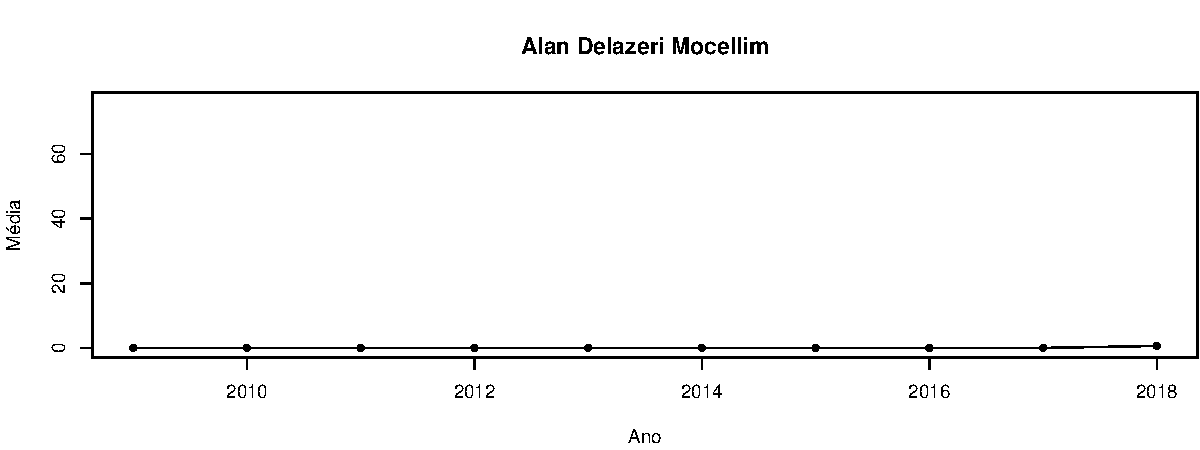
\includegraphics[width=\maxwidth]{figure/mediamovel-1} 

}



\vspace{0.5cm}


{\centering 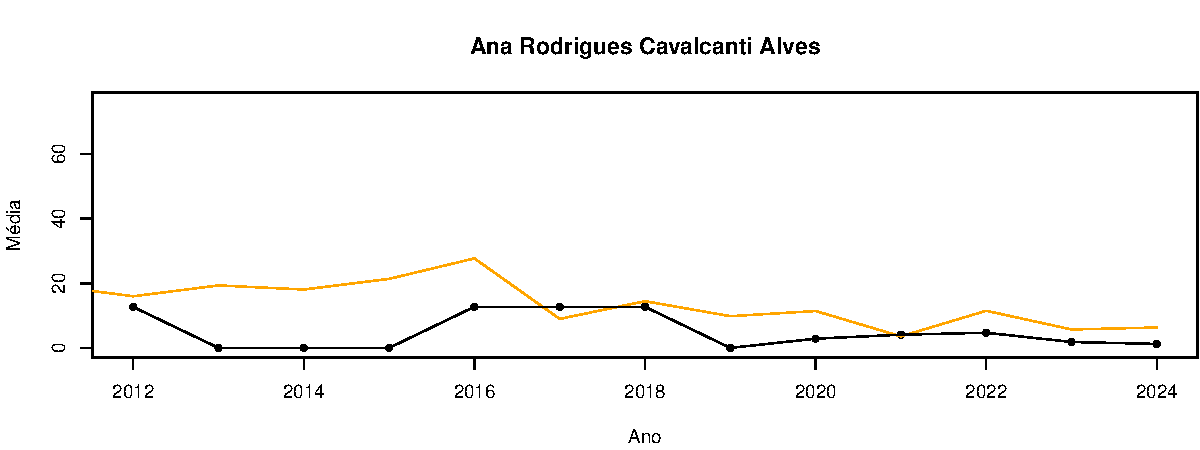
\includegraphics[width=\maxwidth]{figure/mediamovel-2} 

}



\vspace{0.5cm}


{\centering 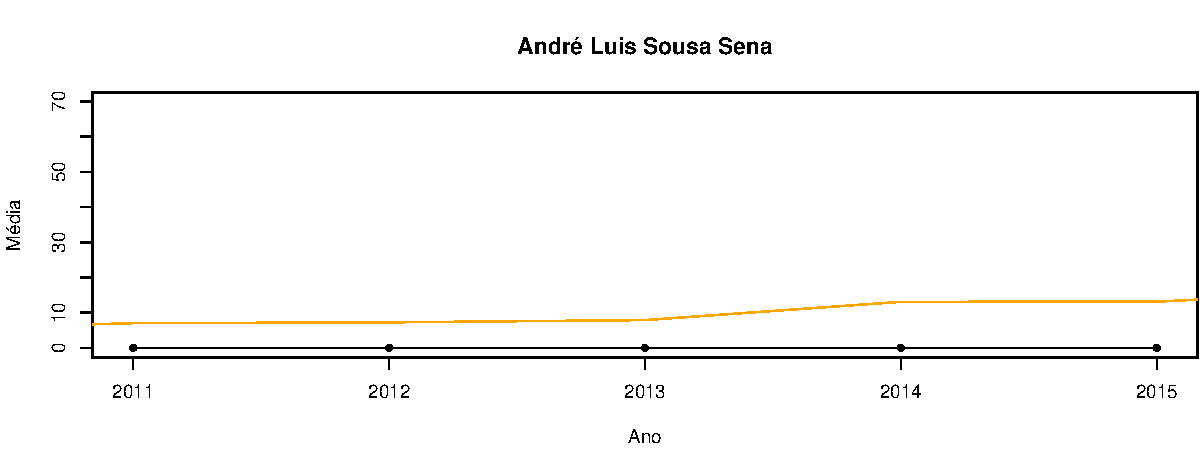
\includegraphics[width=\maxwidth]{figure/mediamovel-3} 

}



\vspace{0.5cm}


{\centering 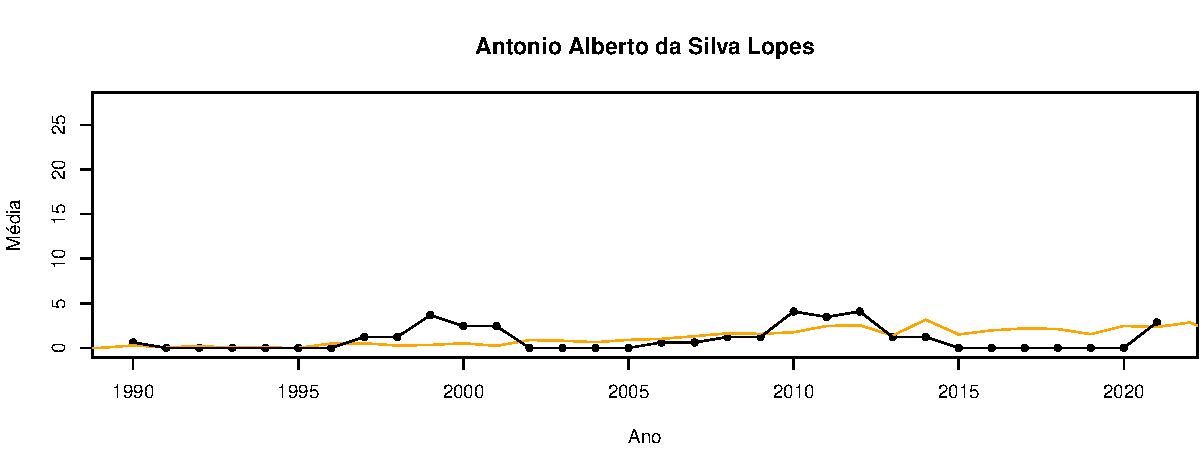
\includegraphics[width=\maxwidth]{figure/mediamovel-4} 

}



\vspace{0.5cm}


{\centering 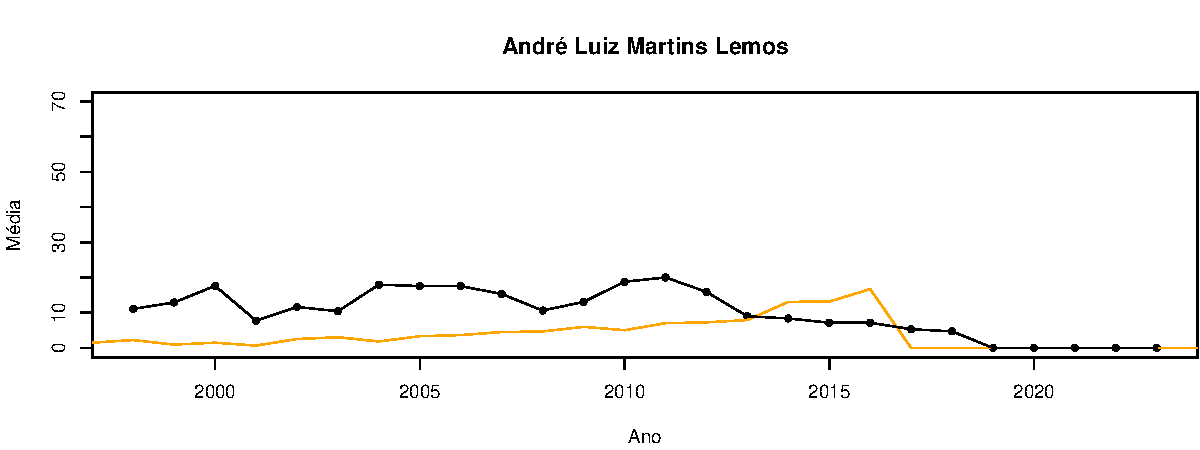
\includegraphics[width=\maxwidth]{figure/mediamovel-5} 

}



\vspace{0.5cm}


{\centering 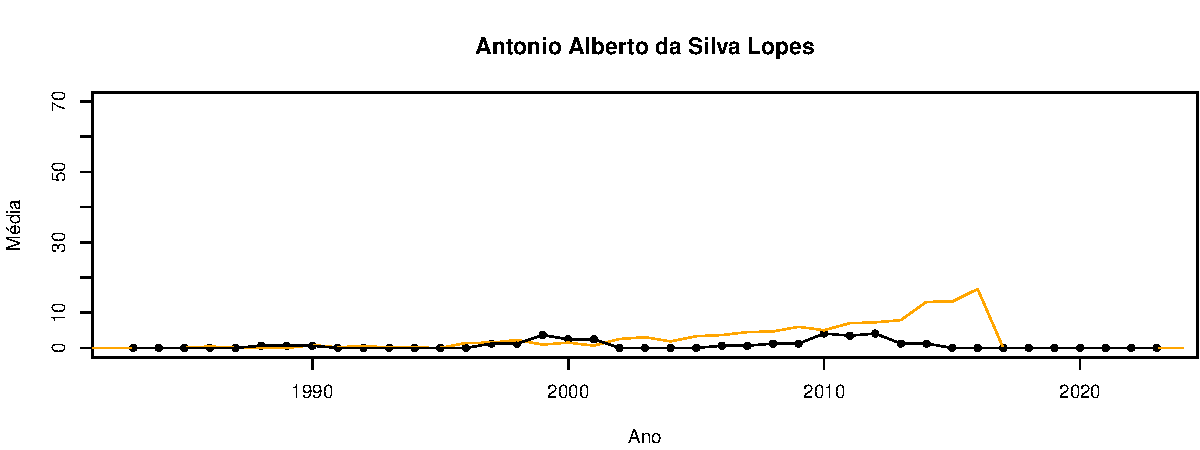
\includegraphics[width=\maxwidth]{figure/mediamovel-6} 

}



\vspace{0.5cm}


{\centering 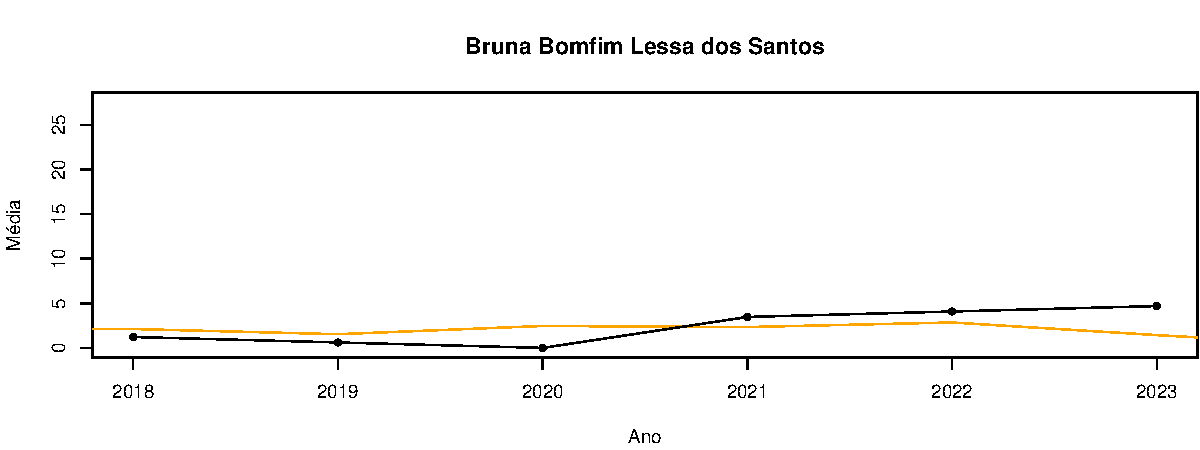
\includegraphics[width=\maxwidth]{figure/mediamovel-7} 

}



\vspace{0.5cm}


{\centering 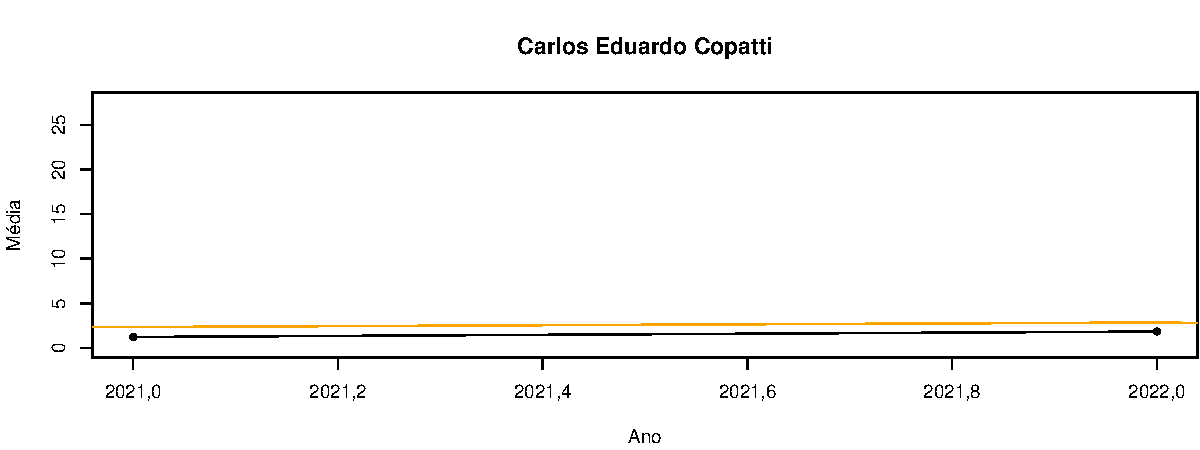
\includegraphics[width=\maxwidth]{figure/mediamovel-8} 

}



\vspace{0.5cm}


{\centering 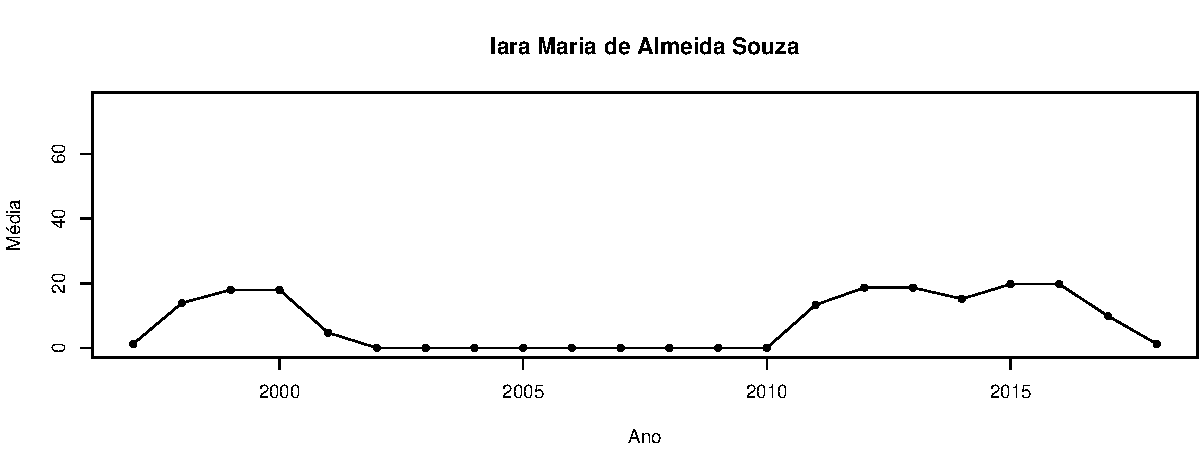
\includegraphics[width=\maxwidth]{figure/mediamovel-9} 

}



\vspace{0.5cm}


{\centering 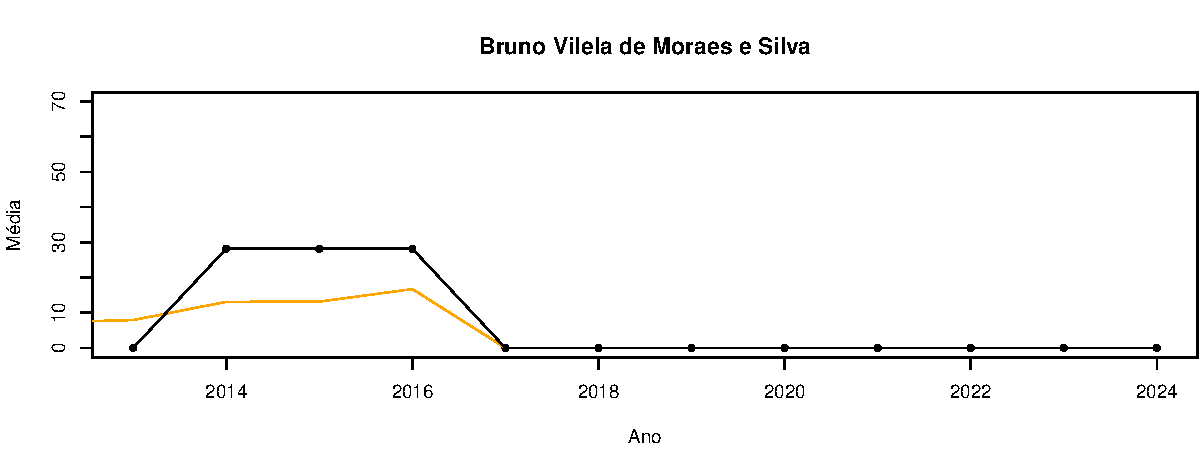
\includegraphics[width=\maxwidth]{figure/mediamovel-10} 

}



\vspace{0.5cm}


{\centering 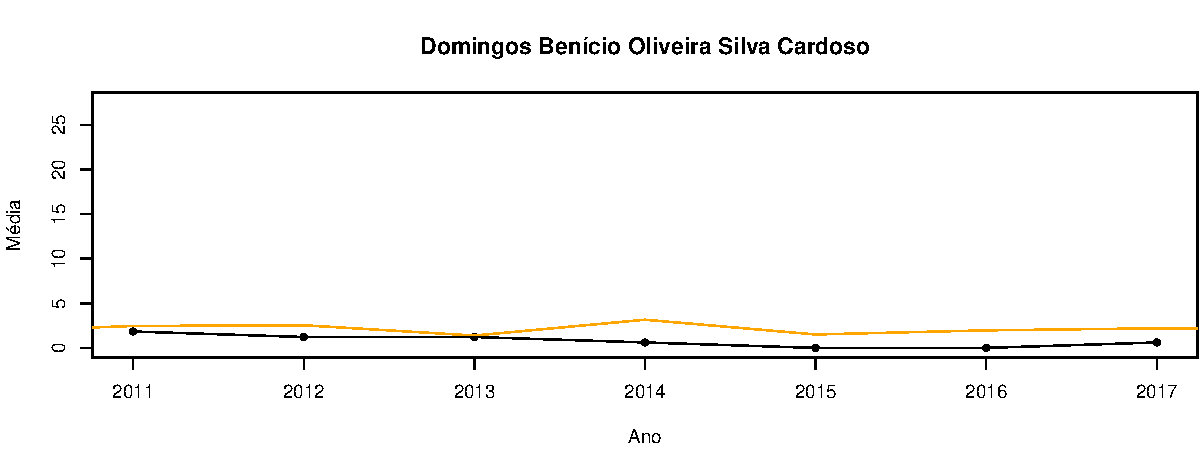
\includegraphics[width=\maxwidth]{figure/mediamovel-11} 

}



\vspace{0.5cm}


{\centering 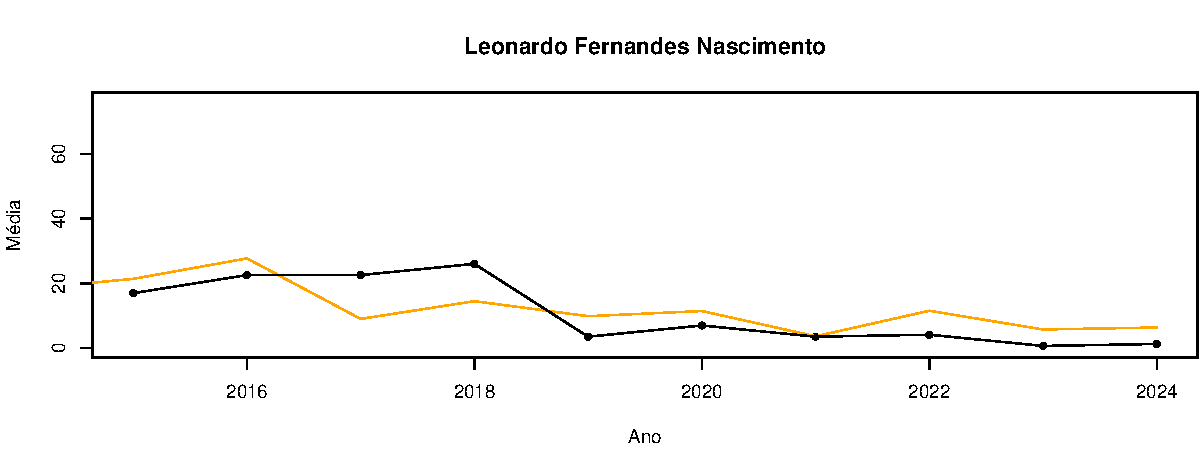
\includegraphics[width=\maxwidth]{figure/mediamovel-12} 

}



\vspace{0.5cm}


{\centering 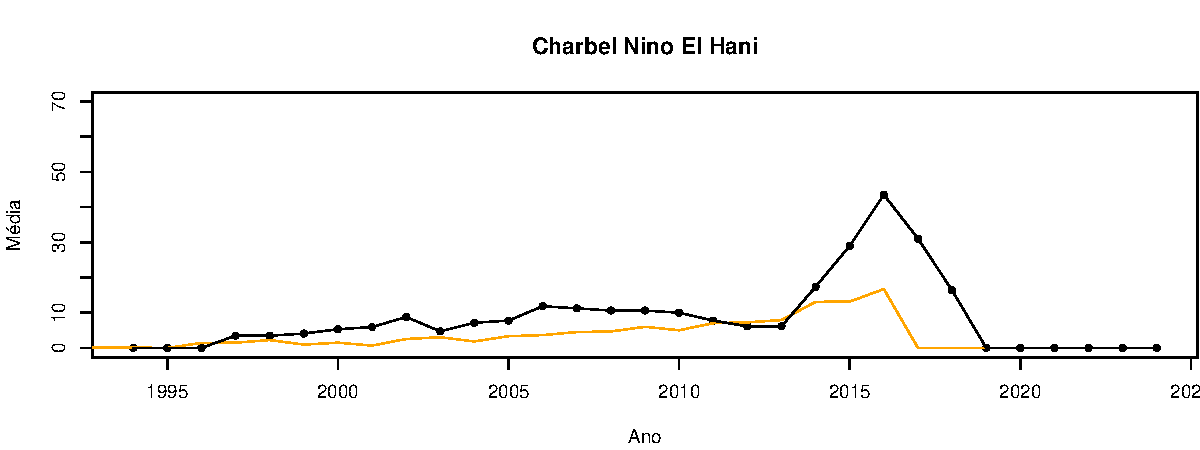
\includegraphics[width=\maxwidth]{figure/mediamovel-13} 

}



\vspace{0.5cm}


{\centering 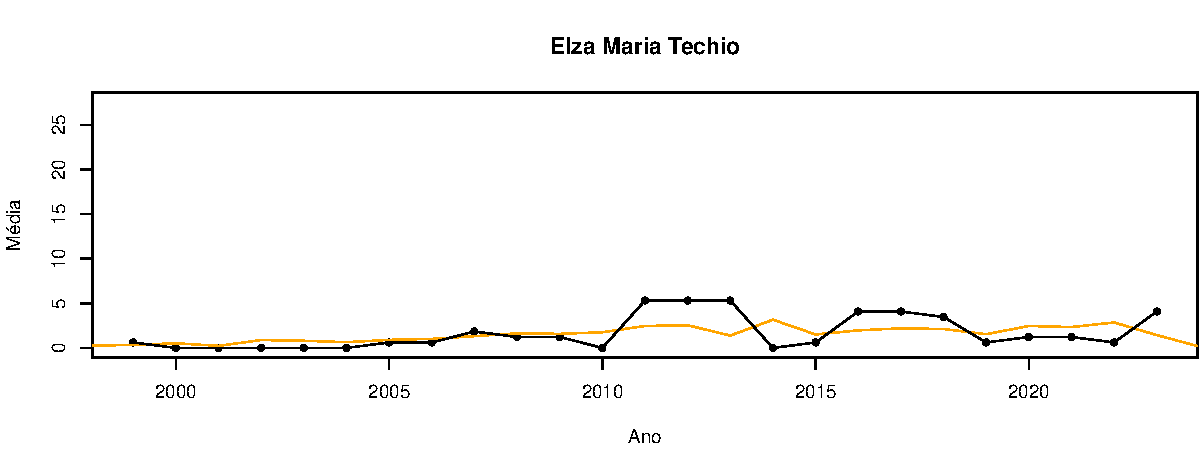
\includegraphics[width=\maxwidth]{figure/mediamovel-14} 

}



\vspace{0.5cm}


{\centering 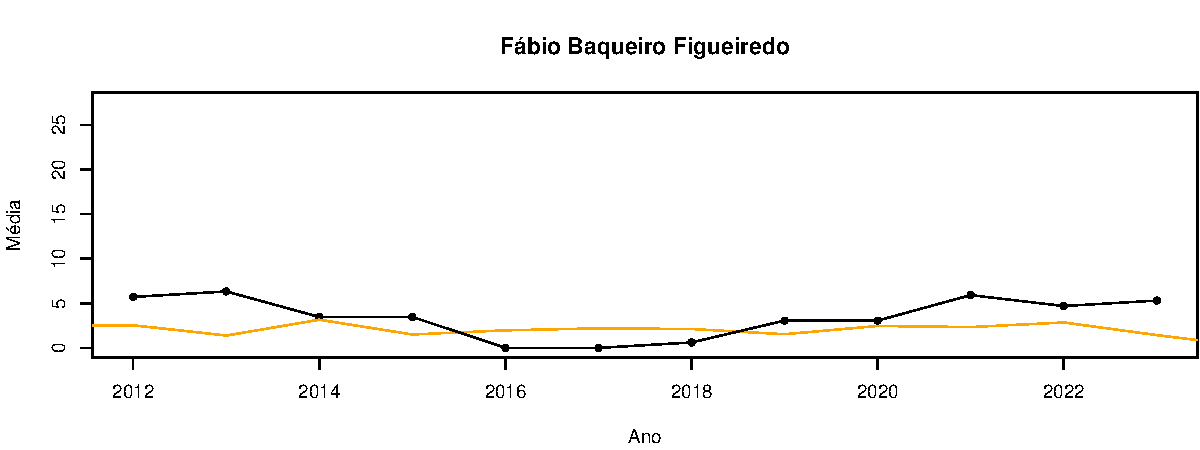
\includegraphics[width=\maxwidth]{figure/mediamovel-15} 

}



\vspace{0.5cm}


{\centering 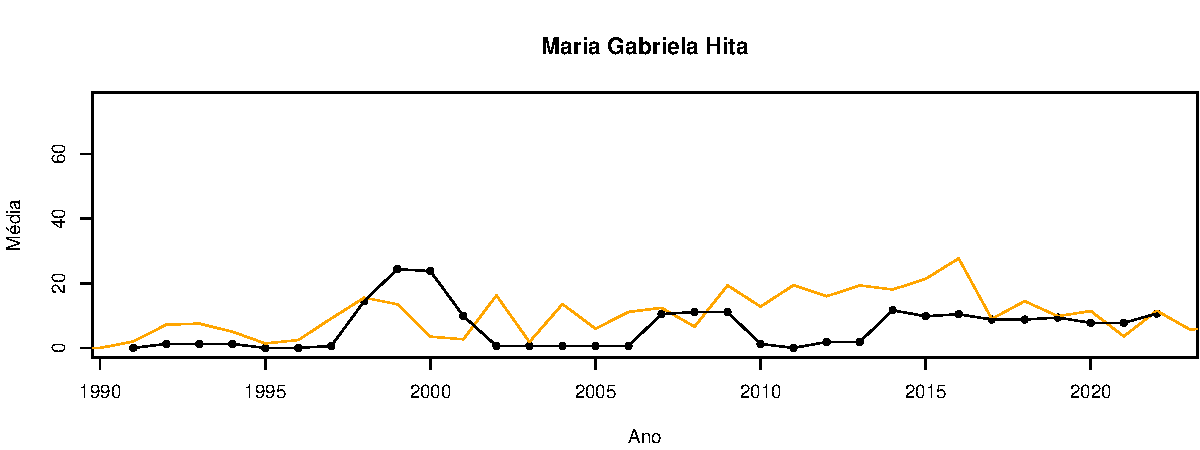
\includegraphics[width=\maxwidth]{figure/mediamovel-16} 

}



\vspace{0.5cm}


{\centering 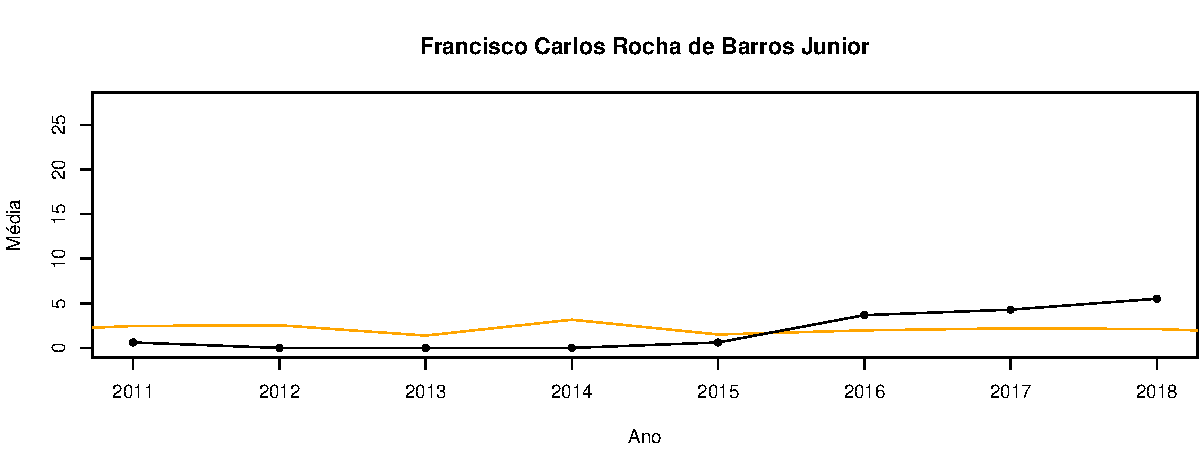
\includegraphics[width=\maxwidth]{figure/mediamovel-17} 

}



\vspace{0.5cm}


{\centering 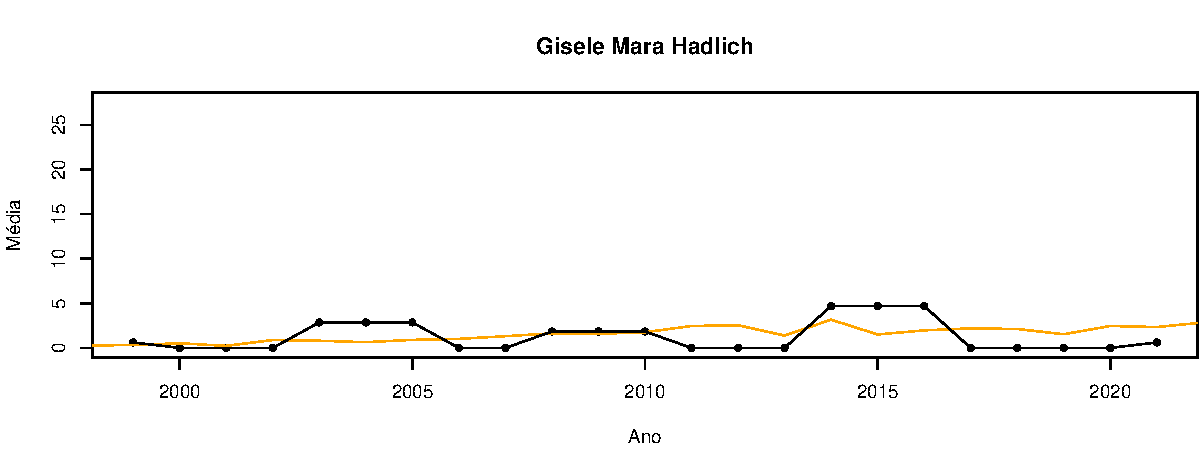
\includegraphics[width=\maxwidth]{figure/mediamovel-18} 

}



\vspace{0.5cm}


{\centering 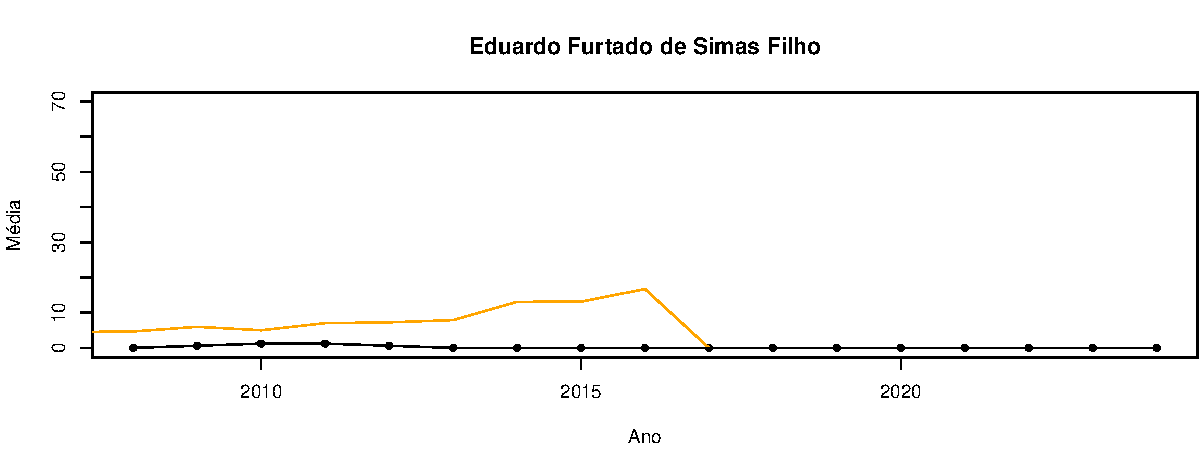
\includegraphics[width=\maxwidth]{figure/mediamovel-19} 

}



\vspace{0.5cm}


{\centering 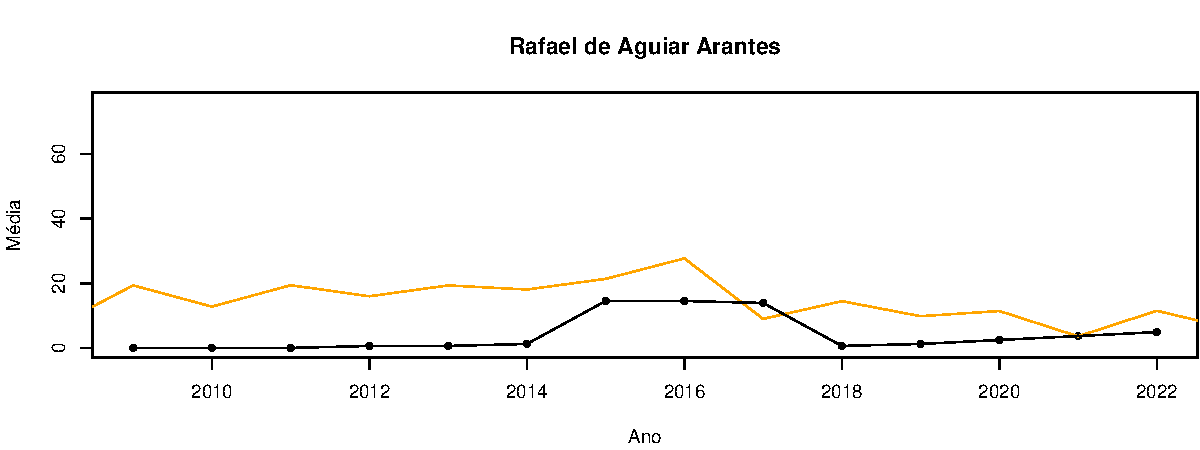
\includegraphics[width=\maxwidth]{figure/mediamovel-20} 

}



\vspace{0.5cm}


{\centering \includegraphics[width=\maxwidth]{figure/mediamovel-21} 

}



\vspace{0.5cm}


{\centering \includegraphics[width=\maxwidth]{figure/mediamovel-22} 

}



\vspace{0.5cm}


\clearpage

\section{Apêndices}

A tabela seguinte lista a produção com coautoria entre professores do
programa e, nas três últimas colunas, mostra o número de autores, sendo a
coautoria identificada de acordo com três métodos:

\vspace{2mm}

\begin{tabular}{crl}
 ~~~~~~~~~ &  \textbf{N} & Nome completo dos autores.\\
 ~~~~~~~~~ &  \textbf{C} & Código do CNPq dos autores.\\
 ~~~~~~~~~ &  \textbf{V} & Coincidência de ISSN/ISBN, ano, tipo de produção (livro, artigo ou capítulo), volume, número e página inicial. \\
\end{tabular}

\phantomsection\stepcounter{tabela}\addcontentsline{lot}{table}{Tabela \thetabela: Trabalhos produzidos em coautoria}
\begin{longtable}{|E{3cm}|E{6cm}|c|E{5cm}|r|r|r|r|}
    \multicolumn{8}{c}{\textbf{Tabela \thetabela: Trabalhos produzidos em coautoria}} \\
    \hline
    \multirow{2}{*}{\textbf{Professor}} & \multirow{2}{*}{\textbf{Produção}} &
    \multirow{2}{*}{\textbf{Ano}} & \multirow{2}{*}{\textbf{Livro ou periódico}} &
    \multirow{2}{*}{\textbf{ISSN ou ISBN}} & \multicolumn{3}{c|}{\textbf{N. Aut.}} \\
    \cline{6-8} & & & & & \textbf{N} & \textbf{C} & \textbf{V} \\
    \hline
    \endfirsthead
    \multicolumn{8}{c}{{\footnotesize ... continuação da página anterior}} \\
    \hline
    \multirow{2}{*}{\textbf{Professor}} & \multirow{2}{*}{\textbf{Produção}} &
    \multirow{2}{*}{\textbf{Ano}} & \multirow{2}{*}{\textbf{Livro ou periódico}} &
    \multirow{2}{*}{\textbf{ISSN ou ISBN}} & \multicolumn{3}{c|}{\textbf{N. Aut.}} \\
    \cline{6-8} & & & & & \textbf{N} & \textbf{C} & \textbf{V} \\
    \endhead
    \hline
    \multicolumn{8}{r}{{\footnotesize Continua na próxima página}} \\
    \endfoot
    \hline
    \endlastfoot
Iara Maria de Almeida Souza & Agência: para além da oposição entre atividade e passividade & 2018 & Políticas etnográficas no campo da ciência e das tecnologias da vida & 9788566094411 & 1 & 1 & 2 \\
\hline
Miriam Cristina Marcilio Rabelo & Agência: para além da oposição entre atividade e passividade & 2018 & Políticas etnográficas no campo da ciência e das tecnologias da vida & 9788566094411 & 1 & 1 & 2 \\
\hline
Mariana Thorstensen Possas & Universidade e ideologia: Ataques às ciências humanas e possibilidades de defesa & 2020 & Em defesa das humanidades & 9786556301471 & 1 & 1 & 2 \\
\hline
Sue Angélica Serra Iamamoto & Universidade e ideologia: reflexões sobre os ataques às ciências humanas e as possibilidades de defesa & 2020 & Em defesa das humanidades & 9786556301471 & 1 & 1 & 2 \\
\hline

\end{longtable}

\clearpage

\textbf{Legenda de informação adicional indicada na tabela seguinte}:

\begin{tabular}{E{23.5cm}}
\rowcolor{coautr}Produção realizada em coautoria por mais de um professor do programa.\\
\end{tabular}


\textbf{Legenda de erros de preenchimento do Lattes indicados na tabela seguinte}:

\begin{tabular}{E{23.5cm}}
\rowcolor{capdup}Capítulo indevidamente registrado porque pertence a livro do próprio professor.\\
\rowcolor{ninval}O ISBN é inválido. Confira se todos os algarismos estão corretos.\\
\rowcolor{duplic}Produção registrada mais de uma vez.\\
\end{tabular}


\small
\label{tab:proddet}
\phantomsection\stepcounter{tabela}\addcontentsline{lot}{table}{Tabela \thetabela: Produção detalhada}
\label{ tab:proddet }
\begin{longtable}{lllrrllrr}
\multicolumn{8}{c}{\textbf{Tabela \thetabela: Produção detalhada}} \\
  \toprule
\textbf{Professor} & \textbf{Produção (títulos truncados)} & \textbf{Ano} & \textbf{Qualis} & \textbf{SJR} & \textbf{SNIP} & \textbf{Periódico ou Livro (títulos truncados)} & \textbf{ISSN/ISBN} \\
\midrule
\endfirsthead
\multicolumn{8}{c}{{\footnotesize ... continuação da página anterior}} \\
  \toprule
\textbf{Professor} & \textbf{Produção (títulos truncados)} & \textbf{Ano} & \textbf{Qualis} & \textbf{SJR} & \textbf{SNIP} & \textbf{Periódico ou Livro (títulos truncados)} & \textbf{ISSN/ISBN} \\
\midrule
\endhead
\midrule
\multicolumn{8}{r}{{\footnotesize Continua na próxima página}} \\
\endfoot
\bottomrule
\endlastfoot
Alan Mocellim & Zygmunt Bauman & 2018 & Cap &  &  & Os sociólogos: de Auguste Comte a Gi & 8532659470 \\
Ana Alves & Com o suor do trabalho: uma anál & 2020 & Lvr &  &  &  & 9786586732917 \\
Antonio Camara & Abordagens sobre a sociologia da & 2018 & Cap &  &  & Ensaios arte e sociedade & 9788523217846 \\
Antonio Camara & Contribuição para uma sociologia & 2018 & Cap &  &  & Ensaios de Sociologia da arte & 9788523217846 \\
Antonio Camara & Ensaios de Sociologia da Arte & 2018 & Org &  &  &  & 9788523217846 \\
Antonio Camara & Pressupostos filosóficos clássic & 2018 & Cap &  &  & Ensaios de Sociologia da Arte & 9788523217846 \\
Antonio Camara & Reflexões para uma sociologia da & 2018 & Cap &  &  & Ensaios de sociologia da arte & 9788523217846 \\
Antonio Camara & ENJEUX ENVIRONNEMENTAUX ET  & 2019 & Org &  &  &  & 9782343180199 \\
Antonio Camara & INTRODUÇÃO & 2019 & Cap &  &  & ENJEUX ENVIRONNEMENTAUX ET  & 9782343180199 \\
Antonio Camara & LE LITTORAL NORD EM IMAGES & 2019 & Cap &  &  & ENJEUX ENVORONNEMENTAUX ET  & 9782343180199 \\
Clóvis Zimmermann & Direitos Humanos na Democracia C & 2018 & Org &  &  &  & 9788570770011 \\
Clóvis Zimmermann & Políticas sociais na perspectiva & 2018 & Cap &  &  & ?Direitos Humanos na Democracia Cont & 9788570770011 \\
\rowcolor{ninval}Clóvis Zimmermann & Estado, proteção social e segura & 2019 & Lvr &  &  &  & 9788523218389 \\
Clóvis Zimmermann & Reformas no Estado de Bem-Estar  & 2019 & Cap &  &  & Estado, proteção social e segurança  & 9788523218379 \\
Eduardo Machado & Vulnerabilidade no ambiente de t & 2017 & Cap &  &  & Escolas em tempo de crise: estudos e & 9788523216528 \\
Eduardo Machado & Governança da segurança como uma & 2020 & Cap &  &  & Meandros da atenção e gestão no enfr & 9786587115047 \\
Elisio Estanque & A classe média à deriva & 2017 & Cap &  &  & Espaços e Tempos em Geografia. Livro & 9789892613482 \\
\rowcolor{duplic}Elisio Estanque & A classe média à deriva & 2018 & Cap &  &  & Espaços e Tempos em Geografia. Livro & 9892613481 \\
Elisio Estanque & Building the ?Contraption?: Anti & 2018 & Cap &  &  & Challenging Austerity: Radical Left  & 9781138211 \\
Elisio Estanque & Caloiros e Doutores: um estudo s & 2018 & Lvr &  &  &  & 9789898536662 \\
Elisio Estanque & Die fliegende Kuh« - Warum Recht & 2018 & Cap &  &  & Arbeiterbewegung von rechts? Ungleic & 9783593509716 \\
Elisio Estanque & Social Movements and Organized L & 2018 & Lvr &  &  &  & 9781472472045 \\
Elisio Estanque & Trade Unions and Social Movement & 2018 & Cap &  &  & Social Movements and Organized Labou & 9781472472 \\
Elisio Estanque & Are Trade Unions in Portugal Tra & 2019 & Cap &  &  & Confronting Crisis and Precariousnes & 9781786610478 \\
Elisio Estanque & Desigualdades, tecnologia e revo & 2019 & Cap &  &  & Desigualdades Sociais e Políticas Pú & 9789897553813 \\
Elisio Estanque & Organizações e desafios sociolab & 2019 & Cap &  &  & Economia social - olhares cruzados & 9789724080680 \\
Elisio Estanque & Praxe e tradição estudantil em C & 2019 & Cap &  &  & Os 31 Desafios para o Ensino Superio & 9789895436125 \\
Elisio Estanque & Tempos conturbados no mundo do t & 2019 & Cap &  &  & Negociação Coletiva - Estado e Desaf & 9789897685866 \\
Felipe Vargas & Controvérsias em biotecnologias  & 2017 & Lvr &  &  &  & 9783330769588 \\
Felipe Vargas & Ambientes entrelaçados: a conser & 2020 & Cap &  &  & Pesquisa em desenvolvimento, ambient & 9788547345792 \\
\rowcolor{coautr}Iara Souza & Agência: para além da oposição e & 2018 & Cap &  &  & Políticas etnográficas no campo da c & 9788566094411 \\
Iara Souza & Metodologia e Teoria Ator-Rede & 2018 & Cap &  &  & Novas Fronteiras Metodológicas nas C & 9788523217976 \\
Iracema Guimarães & Dinâmica Urbana e Contextos de P & 2017 & Cap &  &  & Disputas em Torno do Espaço Urbano.  & 9788523215972 \\
Iracema Guimarães & Apresentação & 2018 & Cap &  &  & CIDADES NO SÉCULO XXI TEMAS & 9788528306088 \\
Iracema Guimarães & CIDADES NO SÉCULO XXI TEMAS & 2018 & Org &  &  &  & 9788528306088 \\
Iracema Guimarães & CIDADES BRASILEIRAS: TEMAS  & 2020 & Org &  &  &  & 9786587387185 \\
\rowcolor{duplic}Iracema Guimarães & Dinâmica Urbana e Contextos de P & 2020 & Cap &  &  & Disputas em torno do espaço urbano:  & 9786556300870 \\
Iracema Guimarães & Reprodução e trabalho & 2020 & Cap &  &  & Dicionário Desenvolvimento e Questão & 9786556840017 \\
Jair Silva & Classes sociais, movimentos soci & 2017 & Cap &  &  & As classes sociais no início do sécu & 9788539108664 \\
Jair Silva & Identidade, diferença e racismo & 2017 & Cap &  &  & Política da promoção da igualdade ra & 9788593527043 \\
Jair Silva & Lutas por reconhecimento, racism & 2017 & Cap &  &  & Cultura afro-brasileira: temas funda & 9788579395031 \\
Jair Silva & Racismo e sindicalismo - reconhe & 2017 & Lvr &  &  &  & 9788539108 \\
Jair Silva & Do sindicalismo de confronto ao  & 2018 & Cap &  &  & O privilégio da servidão: o novo pro & 9788575596296 \\
Jair Silva & Apresentação & 2019 & Cap &  &  & Trabalho, precarização e resistência & 9788523219093 \\
Jair Silva & SINDICALISMO E DIRIGENTES S & 2019 & Cap &  &  & Trabalho, precarização e resistência & 9788523219093 \\
Jair Silva & Trabalho, precarização e resistê & 2019 & Org &  &  &  & 9788523219093 \\
Jair Silva & Sindicalismo e desigualdades rac & 2020 & Cap &  &  & Dicionário Desenvolvimento e Questão & 9786556840017 \\
Jair Silva & TRABALHO, GÊNERO E RACISMO  & 2020 & Cap &  &  & Raça, gênero e classe: : trabalhador & 9786587631172 \\
Leonardo Nascimento & Novas fronteiras metodológicas n & 2018 & Org &  &  &  & 9788523217976 \\
Leonardo Nascimento & O uso do ATLAS.ti na pesqui & 2018 & Cap &  &  & Novas fronteiras metodológicas nas c & 9788523217976 \\
Leonardo Nascimento & A Midiatização do refúgio no Bra & 2020 & Cap &  &  & A Midiatização do refúgio no Brasil  & 9786556350042 \\
Leonardo Nascimento & Sociologia digital: uma breve in & 2020 & Lvr &  &  &  & 9786556301082 \\
Lucas Oliveira & Language and Urban Place & 2017 & Cap &  &  & Oxford Bibliographies in Anthropolog & 9780199766567 \\
Lucas Oliveira & Três comentários sobre certa & 2017 & Cap &  &  & Coleção Literatura Comparada & 9788593243097 \\
Lucas Oliveira & Cultura, política e produção de  & 2019 & Cap &  &  & Literatura e Periferias & 9788580490862 \\
Lucas Oliveira & Experiências Estéticas em Movime & 2020 & Lvr &  &  &  & 9786586657333 \\
Luiz Lourenço & Abrindo a Caixa-Preta: a decisão & 2017 & Lvr &  &  &  & 9783330752078 \\
Luiz Lourenço & Abrindo a caixa-preta: da indeci & 2017 & Cap &  &  & ELEIÇÕES, OPINIÃO PÚBLICA E & 9788575114353 \\
Luiz Lourenço & Direitos humanos na democracia c & 2018 & Org &  &  &  & 9788570770134 \\
Luiz Lourenço & Prisões fora da lei: notas de um & 2018 & Cap &  &  & Direitos humanos na democracia conte & 9788570770134 \\
Maria Faria & A terceirização sem limites: mai & 2017 & Cap &  &  & Saúde e Segurança do Trabalho no Bra & 9788566507157 \\
Maria Faria & Terceirização no serviço público & 2017 & Cap &  &  & O Avesso do Trabalho IV - Terceiriza & 9788594820136 \\
Maria Faria & A hegemonia da individualização  & 2018 & Cap &  &  & Direito Ambiental do Trabalho - apon & 9788536196930 \\
Maria Faria & A Precarização do Trabalho como  & 2018 & Cap &  &  & O Privilégio da Servidão - o novo pr & 9788575596296 \\
Maria Faria & A reforma trabalhista: uma refor & 2018 & Cap &  &  & A Reforma Trabalhosta na visão da Aj & 9788595301108 \\
Maria Faria & A TERCEIRIZAÇÃO NO SERVIÇO  & 2018 & Cap &  &  & erceirização do Trabalho no Brasil:  & 9788578113186 \\
\rowcolor{capdup}Maria Faria & A Contrareforma neoliberal e a t & 2019 & Cap &  &  & Trabalho, Precarização e Resistência & 9788523219093 \\
Maria Faria & Trabalho, Precarização e Resistê & 2019 & Lvr &  &  &  & 9788523219093 \\
Maria Faria & (Verbete)  Precarização social d & 2020 & Cap &  &  & Dicionário Temático Desenvolvimento  & 9786556840017 \\
Maria Faria & O BRASIL NAS TREVAS ( 2013- & 2020 & Lvr &  &  &  & 9786557170304 \\
Maria Hita & Apresentação & 2017 & Cap &  &  & Disputas em torno do Espaço Urbano:  & 9788523215972 \\
Maria Hita & Disputas em torno do Espaço Urba & 2017 & Org &  &  &  & 9788523215972 \\
Maria Hita & Introdução: A questão Urbana Hoj & 2017 & Cap &  &  & Disputas em torno do Espaço Urbano:  & 9788523215972 \\
Maria Hita & Introdução: Controversias e deba & 2017 & Cap &  &  & Raça, racismo e genética em debates  & 9788523215743 \\
Maria Hita & Raça, racismo e genética em deba & 2017 & Org &  &  &  & 9788523215743 \\
Maria Hita & Uma comunidade periférica da cid & 2017 & Cap &  &  & Disputas em torno do Espaço Urbano:  & 9788523215972 \\
Maria Hita & Desarrollo urbano e inseguridad: & 2019 & Cap &  &  & Disputas por el Espacio Urbano: Desi & 9789876915878 \\
Maria Hita & Neighbourhood Grassroots Organiz & 2019 & Cap &  &  & The Routledge Handbook of Anthropolo & 9781138126091 \\
Maria Hita & A desigualdade em clave contínu & 2020 & Cap &  &  & Disputas em torno do espaço urbano  & 9786556300870 \\
Maria Hita & Disputas em torno do espaço urb & 2020 & Org &  &  &  & 9786556300870 \\
Maria Hita & Introdução: a questão urbana, & 2020 & Cap &  &  & Disputas em torno do espaço urbano  & 9786556300870 \\
Maria Hita & Matriarcalidade, questão racial  & 2020 & Cap &  &  & Dicionário Temático Desenvolvimento  & 9786556840017 \\
Maria Hita & Organização de Base Comunitárias & 2020 & Cap &  &  & Modos de Fazer/ Ways of Making & 9789898970237 \\
Maria Hita & Political Parties, Big Business, & 2020 & Cap &  &  & After the Pink Tide: Corporate State & 9781789206593 \\
Maria Hita & Uma comunidade periférica da ci & 2020 & Cap &  &  & Disputas em torno do espaço urbano  & 9786556300870 \\
Mariana Possas & Os direitos humanos como‘discurs & 2018 & Cap &  &  & Direitos Humanos na Democracia Conte & 8570770014 \\
Mariana Possas & A criação da lei do feminicidio  & 2020 & Cap &  &  & A racionalidade penal moderna : refl & 9786556270470 \\
Mariana Possas & A racionalidade penal moderna e  & 2020 & Cap &  &  & A racionalidade penal moderna : refl & 9786556271064 \\
\rowcolor{coautr}Mariana Possas & Universidade e ideologia: Ataque & 2020 & Cap &  &  & Em defesa das humanidades & 9786556301471 \\
\rowcolor{coautr}Miriam Rabelo & Agência: para além da oposição e & 2018 & Cap &  &  & Políticas etnográficas no campo da c & 9788566094411 \\
Miriam Rabelo & Candomblé and the Magic of Bahia & 2018 & Cap &  &  & The Making of Brazil’s Black Mecca B & 9781611862942 \\
Paulo Alves & A modernidade e o caráter sublim & 2017 & Cap &  &  & Disputas em torno do espeço urbano & 9788523215972 \\
\rowcolor{capdup}Paulo Alves & As‘novas sociologias’e a constru & 2018 & Cap &  &  & Novas Fronteiras Metodológicas nas C & 9788523217976 \\
Paulo Alves & Novas Fronteiras Metodológicas n & 2018 & Lvr &  &  &  & 9788523217976 \\
Paulo Alves & A relação entre a teoria socioló & 2020 & Cap &  &  & Campos das Ciências Sociais & 8532663757 \\
Rafael Arantes & Inter-reconhecimento, Diversidad & 2018 & Cap &  &  & Cidades no século XXI: temas em deba & 9788528306088 \\
Rafael Arantes & A restrição dos espaços públicos & 2019 & Cap &  &  & Retratos sul-americanos: perspectiva & 9788572670050 \\
Rafael Arantes & A pandemia da COVID-19 em u & 2020 & Cap &  &  & AS METRÓPOLES E A COVID-19: & 9786500078138 \\
Rafael Arantes & Mercantilização dos espaços públ & 2020 & Cap &  &  & Cidades brasileiras: temas e questõe & 9786587387185 \\
Ricardo Regatieri & Capitalismo e modernidade no“res & 2018 & Cap &  &  & América Latina y Corea del Sur: inte & 9788577323616 \\
Ricardo Regatieri & Capitalismo sem peias: a crítica & 2019 & Lvr &  &  &  & 9788577323814 \\
Sue Iamamoto & Democracia na América Latina 2:  & 2019 & Lvr &  &  &  & 9788593230509 \\
Sue Iamamoto & Nacionalismo & 2020 & Cap &  &  & Dicionário das Eleições & 9786556052441 \\
\rowcolor{coautr}Sue Iamamoto & Universidade e ideologia: reflex & 2020 & Cap &  &  & Em defesa das humanidades & 9786556301471 \\
\end{longtable}

\normalsize

\clearpage

A tabela seguinte tem o objetivo de ajudar a identificar erros de
digitação nos títulos dos periódicos, podendo ser uma diferença tão pequena
quanto uma vogal sem acento. Constam da tabela os títulos com pelo menos uma
letra diferente do título de mesmo ISSN na planilha Qualis. Adicionalmente,
estão realçadas de amarelo as linhas em que não foi possível encontrar uma
sequência idêntica de 12 letras nos dois títulos.

\phantomsection\stepcounter{tabela}\addcontentsline{lot}{table}{Tabela \thetabela: Títulos de periódicos registrados nos currículos com alguma diferença dos títulos na planilha Qualis}
\label{ tab:ttldif }
\begin{ltabulary}{LL}
\multicolumn{2}{c}{\textbf{Tabela \thetabela: Títulos de periódicos registrados nos currículos com alguma diferença dos títulos na planilha Qualis}} \\
  \toprule
\textbf{Título Qualis} & \textbf{Título Lattes} \\
\midrule
\endfirsthead
\multicolumn{2}{c}{{\footnotesize ... continuação da página anterior}} \\
  \toprule
\textbf{Título Qualis} & \textbf{Título Lattes} \\
\midrule
\endhead
\midrule
\multicolumn{2}{r}{{\footnotesize Continua na próxima página}} \\
\endfoot
\bottomrule
\endlastfoot
 \\
\end{ltabulary}


\clearpage

Periódicos podem estar sem Qualis porque não foram ainda classificados pelo
comitê da área ou porque o professor errou a digitação do ISSN no currículo
Lattes. Para descobrir se foi um erro de digitação, veja na
tabela da produção detalhada (página~\pageref{tab:proddet}) quem foi o professor que publicou no periódico,
descubra qual o ISSN correto do periódico e verifique no currículo Lattes do
professor se os dados foram digitados corretamente.

\phantomsection\stepcounter{tabela}\addcontentsline{lot}{table}{Tabela \thetabela: Lista de periódicos sem qualis}
\begin{ltabulary}{lL}
\multicolumn{2}{c}{\textbf{Tabela \thetabela: Lista de periódicos sem qualis}} \\
  \toprule
\textbf{ISSN} & \textbf{Título do periódico} \\
\midrule
\endfirsthead
\multicolumn{2}{c}{{\footnotesize ... continuação da página anterior}} \\
  \toprule
\textbf{ISSN} & \textbf{Título do periódico} \\
\midrule
\endhead
\midrule
\multicolumn{2}{r}{{\footnotesize Continua na próxima página}} \\
\endfoot
\bottomrule
\endlastfoot
 \\
\end{ltabulary}


\end{document}
